%! TEX root = main.tex

%----------------------------------------------------------------------------------------
%	PACKAGES AND OTHER DOCUMENT CONFIGURATIONS
%----------------------------------------------------------------------------------------

\documentclass[
	9pt, % Set the default font size, options include: 8pt, 9pt, 10pt, 11pt, 12pt, 14pt, 17pt, 20pt
	% t, % Uncomment to vertically align all slide content to the top of the slide, rather than the default centered
	% aspectratio=169, % Uncomment to set the aspect ratio to a 16:9 ratio which matches the aspect ratio of 1080p and 4K screens and projectors
]{beamer}

% Use German lang
% \usepackage[ngerman]{babel}

% \graphicspath{{Images/}{./}} % Specifies where to look for included images (trailing slash required)
\usepackage{hyperref}
\usepackage{multimedia}
\usepackage{booktabs} % Allows the use of \toprule, \midrule and \bottomrule for better rules in tables
\usepackage{physics}
\usepackage{siunitx}
\usepackage[outputdir=build]{minted}

%----------------------------------------------------------------------------------------
%	SELECT LAYOUT THEME
%----------------------------------------------------------------------------------------

% Beamer comes with a number of default layout themes which change the colors and layouts of slides. Below is a list of all themes available, uncomment each in turn to see what they look like.

% \usetheme{default}
% \usetheme{AnnArbor}
%\usetheme{Antibes}
% \usetheme{Bergen} % quite modern, use this probably
% \usetheme{Berkeley}
% \usetheme{Berlin}
% \usetheme{Boadilla}
% \usetheme{CambridgeUS}
% \usetheme{Copenhagen}
% \usetheme{Darmstadt}
% \usetheme{Dresden}
% \usetheme{Frankfurt}
% \usetheme{Goettingen}
\usetheme{Hannover} % quite nice as well
% \usetheme{Ilmenau}
% \usetheme{JuanLesPins}
% \usetheme{Luebeck}
% \usetheme{Madrid}
% \usetheme{Malmoe}
% \usetheme{Marburg}
% \usetheme{Montpellier}
% \usetheme{PaloAlto}
% \usetheme{Pittsburgh}
% \usetheme{Rochester}
% \usetheme{Singapore}
% \usetheme{Szeged}
% \usetheme{Warsaw}

%----------------------------------------------------------------------------------------
%	SELECT COLOR THEME
%----------------------------------------------------------------------------------------

% Beamer comes with a number of color themes that can be applied to any layout theme to change its colors.
% Uncomment each of these in turn to see how they change the colors of your selected layout theme.

% \usecolortheme{albatross}
% \usecolortheme{beaver}
% \usecolortheme{beetle}
% \usecolortheme{crane}
\usecolortheme{dolphin}
%\usecolortheme{dove}
%\usecolortheme{fly}
%\usecolortheme{lily}
%\usecolortheme{monarca}
%\usecolortheme{seagull}
%\usecolortheme{seahorse}
%\usecolortheme{spruce}
%\usecolortheme{whale}
%\usecolortheme{wolverine}

%----------------------------------------------------------------------------------------
%	SELECT FONT THEME & FONTS
%----------------------------------------------------------------------------------------

% Beamer comes with several font themes to easily change the fonts used in various parts of the presentation. Review the comments beside each one to decide if you would like to use it. Note that additional options can be specified for several of these font themes, consult the beamer documentation for more information.

\usefonttheme{default} % Typeset using the default sans serif font
%\usefonttheme{serif} % Typeset using the default serif font (make sure a sans font isn't being set as the default font if you use this option!)

%------------------------------------------------

\usepackage{mathptmx} % Use the Times font for serif text
% \usepackage{palatino} % Use the Palatino font for serif text

% \usepackage{helvet} % Use the Helvetica font for sans serif text
% \usepackage[default]{opensans} % Use the Open Sans font for sans serif text
% \usepackage[default]{FiraSans} % Use the Fira Sans font for sans serif text
\usepackage[default]{FiraSans} % Use the Fira Sans font for sans serif text
% \usepackage[default]{lato} % Use the Lato font for sans serif text

%----------------------------------------------------------------------------------------
%	SELECT INNER THEME
%----------------------------------------------------------------------------------------

% Inner themes change the styling of internal slide elements, for example: bullet points, blocks, bibliography entries, title pages, theorems, etc. Uncomment each theme in turn to see what changes it makes to your presentation.

% \useinnertheme{default}
% \useinnertheme{circles}
\useinnertheme{rectangles}
% \useinnertheme{rounded}
% \useinnertheme{inmargin}

%----------------------------------------------------------------------------------------
%	SELECT OUTER THEME
%----------------------------------------------------------------------------------------

% Outer themes change the overall layout of slides, such as: header and footer lines, sidebars and slide titles. Uncomment each theme in turn to see what changes it makes to your presentation.

\useoutertheme{default}
% \useoutertheme{infolines}
% \useoutertheme{miniframes}
% \useoutertheme{smoothbars}
% \useoutertheme{sidebar}
% \useoutertheme{split}
% \useoutertheme{shadow}
% \useoutertheme{tree}
% \useoutertheme{smoothtree}

%\setbeamertemplate{footline} % Uncomment this line to remove the footer line in all slides
%\setbeamertemplate{footline}[page number] % Uncomment this line to replace the footer line in all slides with a simple slide count

%\setbeamertemplate{navigation symbols}{} % Uncomment this line to remove the navigation symbols from the bottom of all slides

%----------------------------------------------------------------------------------------
%	PRESENTATION INFORMATION
%----------------------------------------------------------------------------------------

\title[AST245]{AST245 Computational Astrophysics} % The short title in the optional parameter appears at the bottom of every slide, the full title in the main parameter is only on the title page

\subtitle{Treecode-based: N-Body Simulation} % Presentation subtitle, remove this command if a subtitle isn't required

\author[Armin R. Veres]{Armin Richard Veres\\ 20-700-118} % Presenter name(s), the optional parameter can contain a shortened version to appear on the bottom of every slide, while the main parameter will appear on the title slide

% \institute[UC]{Institut für Informatik, \\ Universität Zürich \\ \smallskip \textit{}} % Your institution, the optional parameter can be used for the institution shorthand and will appear on the bottom of every slide after author names, while the required parameter is used on the title slide and can include your email address or additional information on separate lines

% \date{\today}
\date{January 30, 2024}

%----------------------------------------------------------------------------------------

\DeclareSIUnit \h {\ensuremath{\mathit{h}}}
\DeclareSIUnit \parsec {pc}
\DeclareSIUnit \solarmass {M_\odot}
\DeclareSIUnit \year {yr}

\begin{document}

%----------------------------------------------------------------------------------------
%	TITLE SLIDE
%----------------------------------------------------------------------------------------

\begin{frame}
	\titlepage % Output the title slide, automatically created using the text entered in the PRESENTATION INFORMATION block above
\end{frame}

%----------------------------------------------------------------------------------------
%	TABLE OF CONTENTS SLIDE
%----------------------------------------------------------------------------------------

% The table of contents outputs the sections and subsections that appear in your presentation, specified with the standard \section and \subsection commands. You may either display all sections and subsections on one slide with \tableofcontents, or display each section at a time on subsequent slides with \tableofcontents[pausesections]. The latter is useful if you want to step through each section and mention what you will discuss.

\begin{frame}
	% \frametitle{Presentation Overview} % Slide title, remove this command for no title
	\tableofcontents % Output the table of contents (all sections on one slide)
	%\tableofcontents[pausesections] % Output the table of contents (break sections up across separate slides)
\end{frame}

%----------------------------------------------------------------------------------------
%	PRESENTATION BODY SLIDES
%----------------------------------------------------------------------------------------

\section{Introduction} % Sections are added in order to organize your presentation into discrete blocks, all sections and subsections are automatically output to the table of contents as an overview of the talk but NOT output in the presentation as separate slides

\begin{frame}{Preliminaries}
	\begin{columns}[T] % The "T" option aligns the columns' content at the top
		% Left column
		\begin{column}{0.5\textwidth} % Adjust the width of the column as you like
			\begin{itemize}
				\item C++ based implementation using \texttt{OpenMP} and \texttt{Eigen3}.
				\item \texttt{main.cpp} as center of application
				\item \texttt{particle.c/hpp} Holds Particle3D class with relevant members
				\item \texttt{data.c/hpp} reads in file
				\item \texttt{histogram.c/hpp} and \texttt{shell.c/hpp} handle histogram creation and binning
				\item \texttt{system.c/hpp} Relevant and global constants and factors
				\item \texttt{treecode.c/hpp} Multipole expansion related class and methods
			\end{itemize}
		\end{column}

		% Right column
		\begin{column}{0.5\textwidth} % Adjust the width of the column as you like
			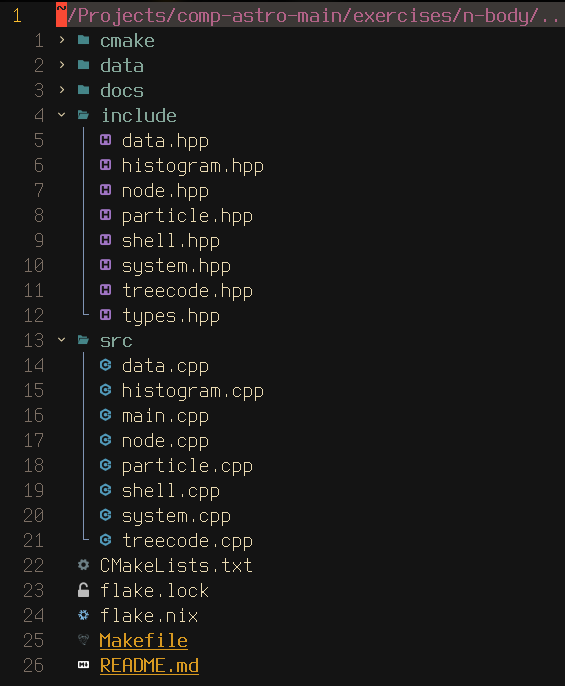
\includegraphics[width=\textwidth]{figures/source-tree}
		\end{column}
	\end{columns}
\end{frame}

\begin{frame}{Units and Dimension}
	From assumption $G=1$ follows: \\
	Dimensionless Quantities:
	\begin{equation}
		\vb{r}^{\prime}=\frac{\vb{r}}{R_0}, \quad m^{\prime}=\frac{m}{M_0}, \quad t^{\prime}=\frac{t}{T_0}
	\end{equation}
	Derived quantities for consistency:
	\begin{equation}
		\begin{aligned}
			\vb{v}^{\prime} = \frac{\vb{v}}{V_0} = \vb{v} \frac{T_0}{R_0}, \quad \vb{a}^{\prime} = \frac{\vb{a}}{A_0} = \vb{a} \frac{T_0^2}{R_0}
		\end{aligned}
	\end{equation}
	Repercussions for setting $G = 1$
	\begin{equation}
		\begin{aligned}
			\vb{a}_i                      & =-G \sum_{j\neq i} m_j \frac{\vb{r}_i-\vb{r}_j}{\left|\vb{r}_i-\vb{r}_j\right|^3} \\
			\Rightarrow \vb{a}_i^{\prime} & =\underbrace{\left\{\frac{G M_0
					T_0^2}{R_0^3}\right\}}_{G^{\prime}} \sum_{j\neq i} m_j^\prime
			\frac{\vb{r}_i^\prime-\vb{r}^\prime_j}{\left|\vb{r}^\prime_i-\vb{r}^\prime_j\right|^3}
		\end{aligned}
	\end{equation}
\end{frame}

\begin{frame}{Defining Units}
	Time scaling factor $T_0$:
	\begin{equation}
		\frac{G M_0 T_0^2}{R_0^3}=1 \quad \Rightarrow \quad T_0=\left(\frac{R_0^3}{G M_0}\right)^{1 / 2}
	\end{equation}\bigskip

	Where:
	\begin{itemize}
		\item $T_0 \simeq 14.91 Myr$
		\item $M_0 =  1 M_\odot$.
		\item $R_0 =  1 pc$.
		\item $V_0 \simeq 0.065 \frac{km}{s} \simeq 0.067 \frac{pc}{Myr}$
		\item $A_0 \simeq 0.004 \frac{pc}{Myr^2}$
	\end{itemize}
	% Data from file assumed as $M_\odot$, $pc$ and $\frac{km}{s}$
\end{frame}

\section{Task 1}
\subsection{Step 1: Density Verification}

\begin{frame}{Analytic Hernquist}

	Density distribution:
	\begin{equation}
		\rho(r) = \frac{M}{2\pi}\frac{a}{r}\frac{1}{(r+a)^3}
		\label{eq:density-distribution}
	\end{equation}

	Cumulative Mass distribution inside a radius:
	\begin{equation}
		M(r) = M \frac{r^2}{(r+a)^2}
		\label{eq:cumulative-mass-distribution}
	\end{equation}

	Reformed Half-mass-radius equation, to get scale length
	\begin{equation}
		a = \frac{r_{1/2}}{1+\sqrt 2}
		\label{eq:scaling length}
	\end{equation}

	{\footnotesize Where:
	\begin{itemize}
		\item $M$  - Total mass of the system
		\item $a$ - Scale Length
		\item $r$ - Particle position vector
		\item $r_{1/2}$ - Half-mass radius: calculated numerically
	\end{itemize}}
\end{frame}

% since all particles have masses of 92. we assumed a mass of 1, to further simplify our equations
\begin{frame}{Numerical Density Approximation}
	Logarithmic binning of particles via \texttt{Histogram} class into a \texttt{std::vector} of \texttt{Shell}
	classes.
	\begin{equation}
		i_{log} = |\vb{r}|_{min} (\frac{|\vb{r}|_{max}}{|\vb{r}|_{min}})^{\frac {i_{lin}}{n}}
		\label{eq:lin-to-log}
	\end{equation}

	On histogram creation calculated for each shell:
	\begin{equation}
		\rho_i = M_i / V_i
		\label{eq:numeric-density}
	\end{equation}

	Poissonian density error with $\sigma = \sqrt{N / B}$:
	\begin{equation}
		\rho_{err} = \frac{\sigma}{V_i}
		\label{eq:density-error}
	\end{equation}

	{\footnotesize Where:
	\begin{itemize}
		\item $i$ - Shell index
		\item $B$ - Number of bins in histogram
		\item $N$ - Number of Particles
	\end{itemize}}

\end{frame}

\begin{frame}{Units}
	From assumption $G=1$ follows:

	\begin{itemize}
		\item $m$ - Mass per particle in Solar Masses (\si{\solarmass})
		\item $r$ - Position / length assumed as is, in Parsecs (\si{\parsec})
		\item $v$ - Velocity, assumed in \si{\kilo\metre\per\second} or \si{\parsec\per\year}
	\end{itemize}
\end{frame}

\begin{frame}
	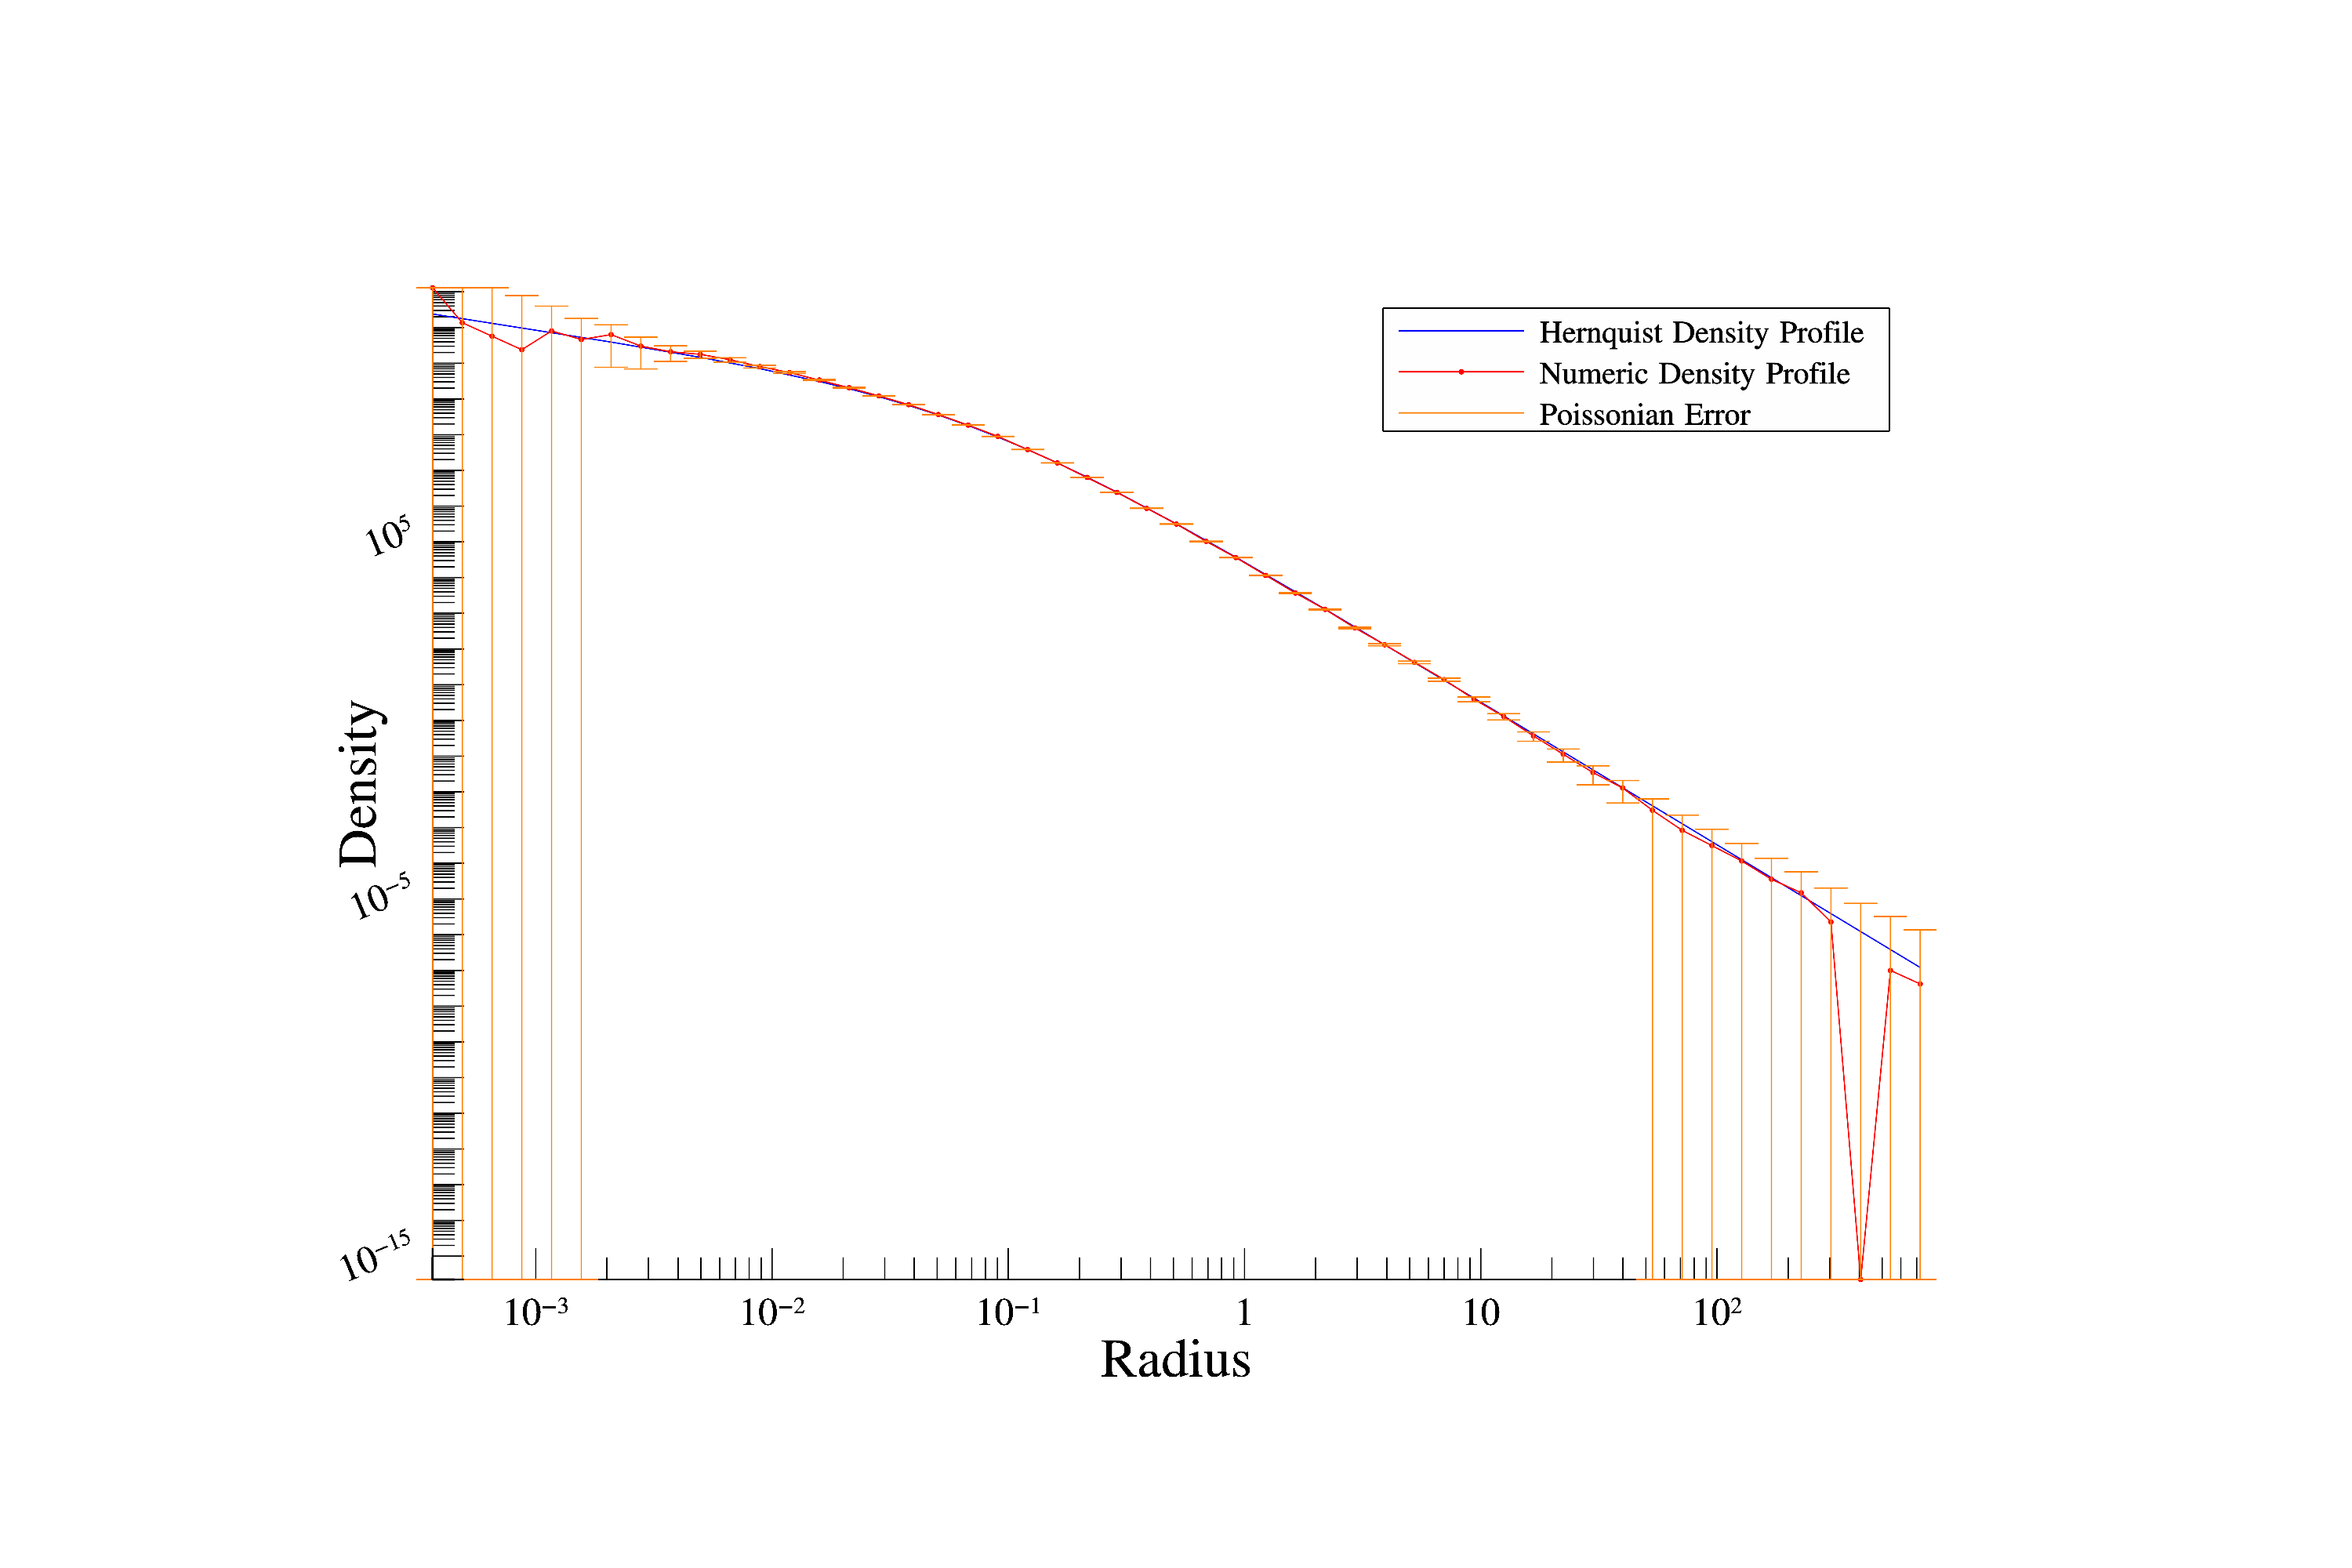
\includegraphics[width=.95\textwidth]{figures/plots/hernquist.png}
\end{frame}

\subsection{Step 2: Direct Force Calculation}
\begin{frame}{Step 2: Analytic Force Reference}

	Taken from \cite{2008gady}, substituting $M(r)$ from Eq. (\ref{eq:cumulative-mass-distribution}) and
	reducing:
	\begin{equation}
		F(r) = - \frac{GM(r)}{r^2} \Rightarrow F(r) = - \frac{M}{(r+a)^2}
		\label{eq:newton-force}
	\end{equation}

	{\footnotesize Where:
	\begin{itemize}
		\item $M$ - Total Mass of System
		\item $r$ - Radius of shell
		\item $a$ - Scale length of System
	\end{itemize}}
\end{frame}

\begin{frame}{Step 2: Direct Force Calculation}
	\begin{equation}
		F_i=-G m_i \sum_{j=1}^N \frac{m_j}{\left[\left(\vb{r}_i-\vb{r}_j\right)^2+\varepsilon^2\right]^{3 /
				2}}\left(\vb{r}_i-\vb{r}_j\right)
		\label{eq:direct-force-full}
	\end{equation}

	% After applying assumptions
	% \begin{equation}
	% 	F_i = - \sum_{j=1}^N \frac{\left(\vb{r}_i-\vb{r}_j\right)}{\left[\left(\vb{r}_i-\vb{r}_j\right)^2+\varepsilon^2\right]^{3 /
	% 			2}}
	% 	\label{eq:direct-force-simple}
	% \end{equation}

	Taken from \cite{2008gady}, equation (2.227)
	\begin{equation}
		% \epsilon=-\frac{r_{max}^2+\frac{3}{2} d^2}{\left(r_{max}^2+d^2\right)^{3 / 2}}
		\epsilon=-\frac{r_{max}^2+\frac{3}{2} a^2}{\left(r_{max}^2+a^2\right)^{3 / 2}}
		\label{eq:softening}
	\end{equation}

	{\footnotesize Where:
	\begin{itemize}
		\item $i$ - Particle under consideration
		\item $\epsilon$ - Softening
		\item $r_{max}$ - Maximum radius
		      % \item $d$ - Mean inter-particle separation, calculated numerically once
		\item $a$ - Scale length
		\item $G=1$
	\end{itemize} }
\end{frame}

\begin{frame}{Softening /= 1}
	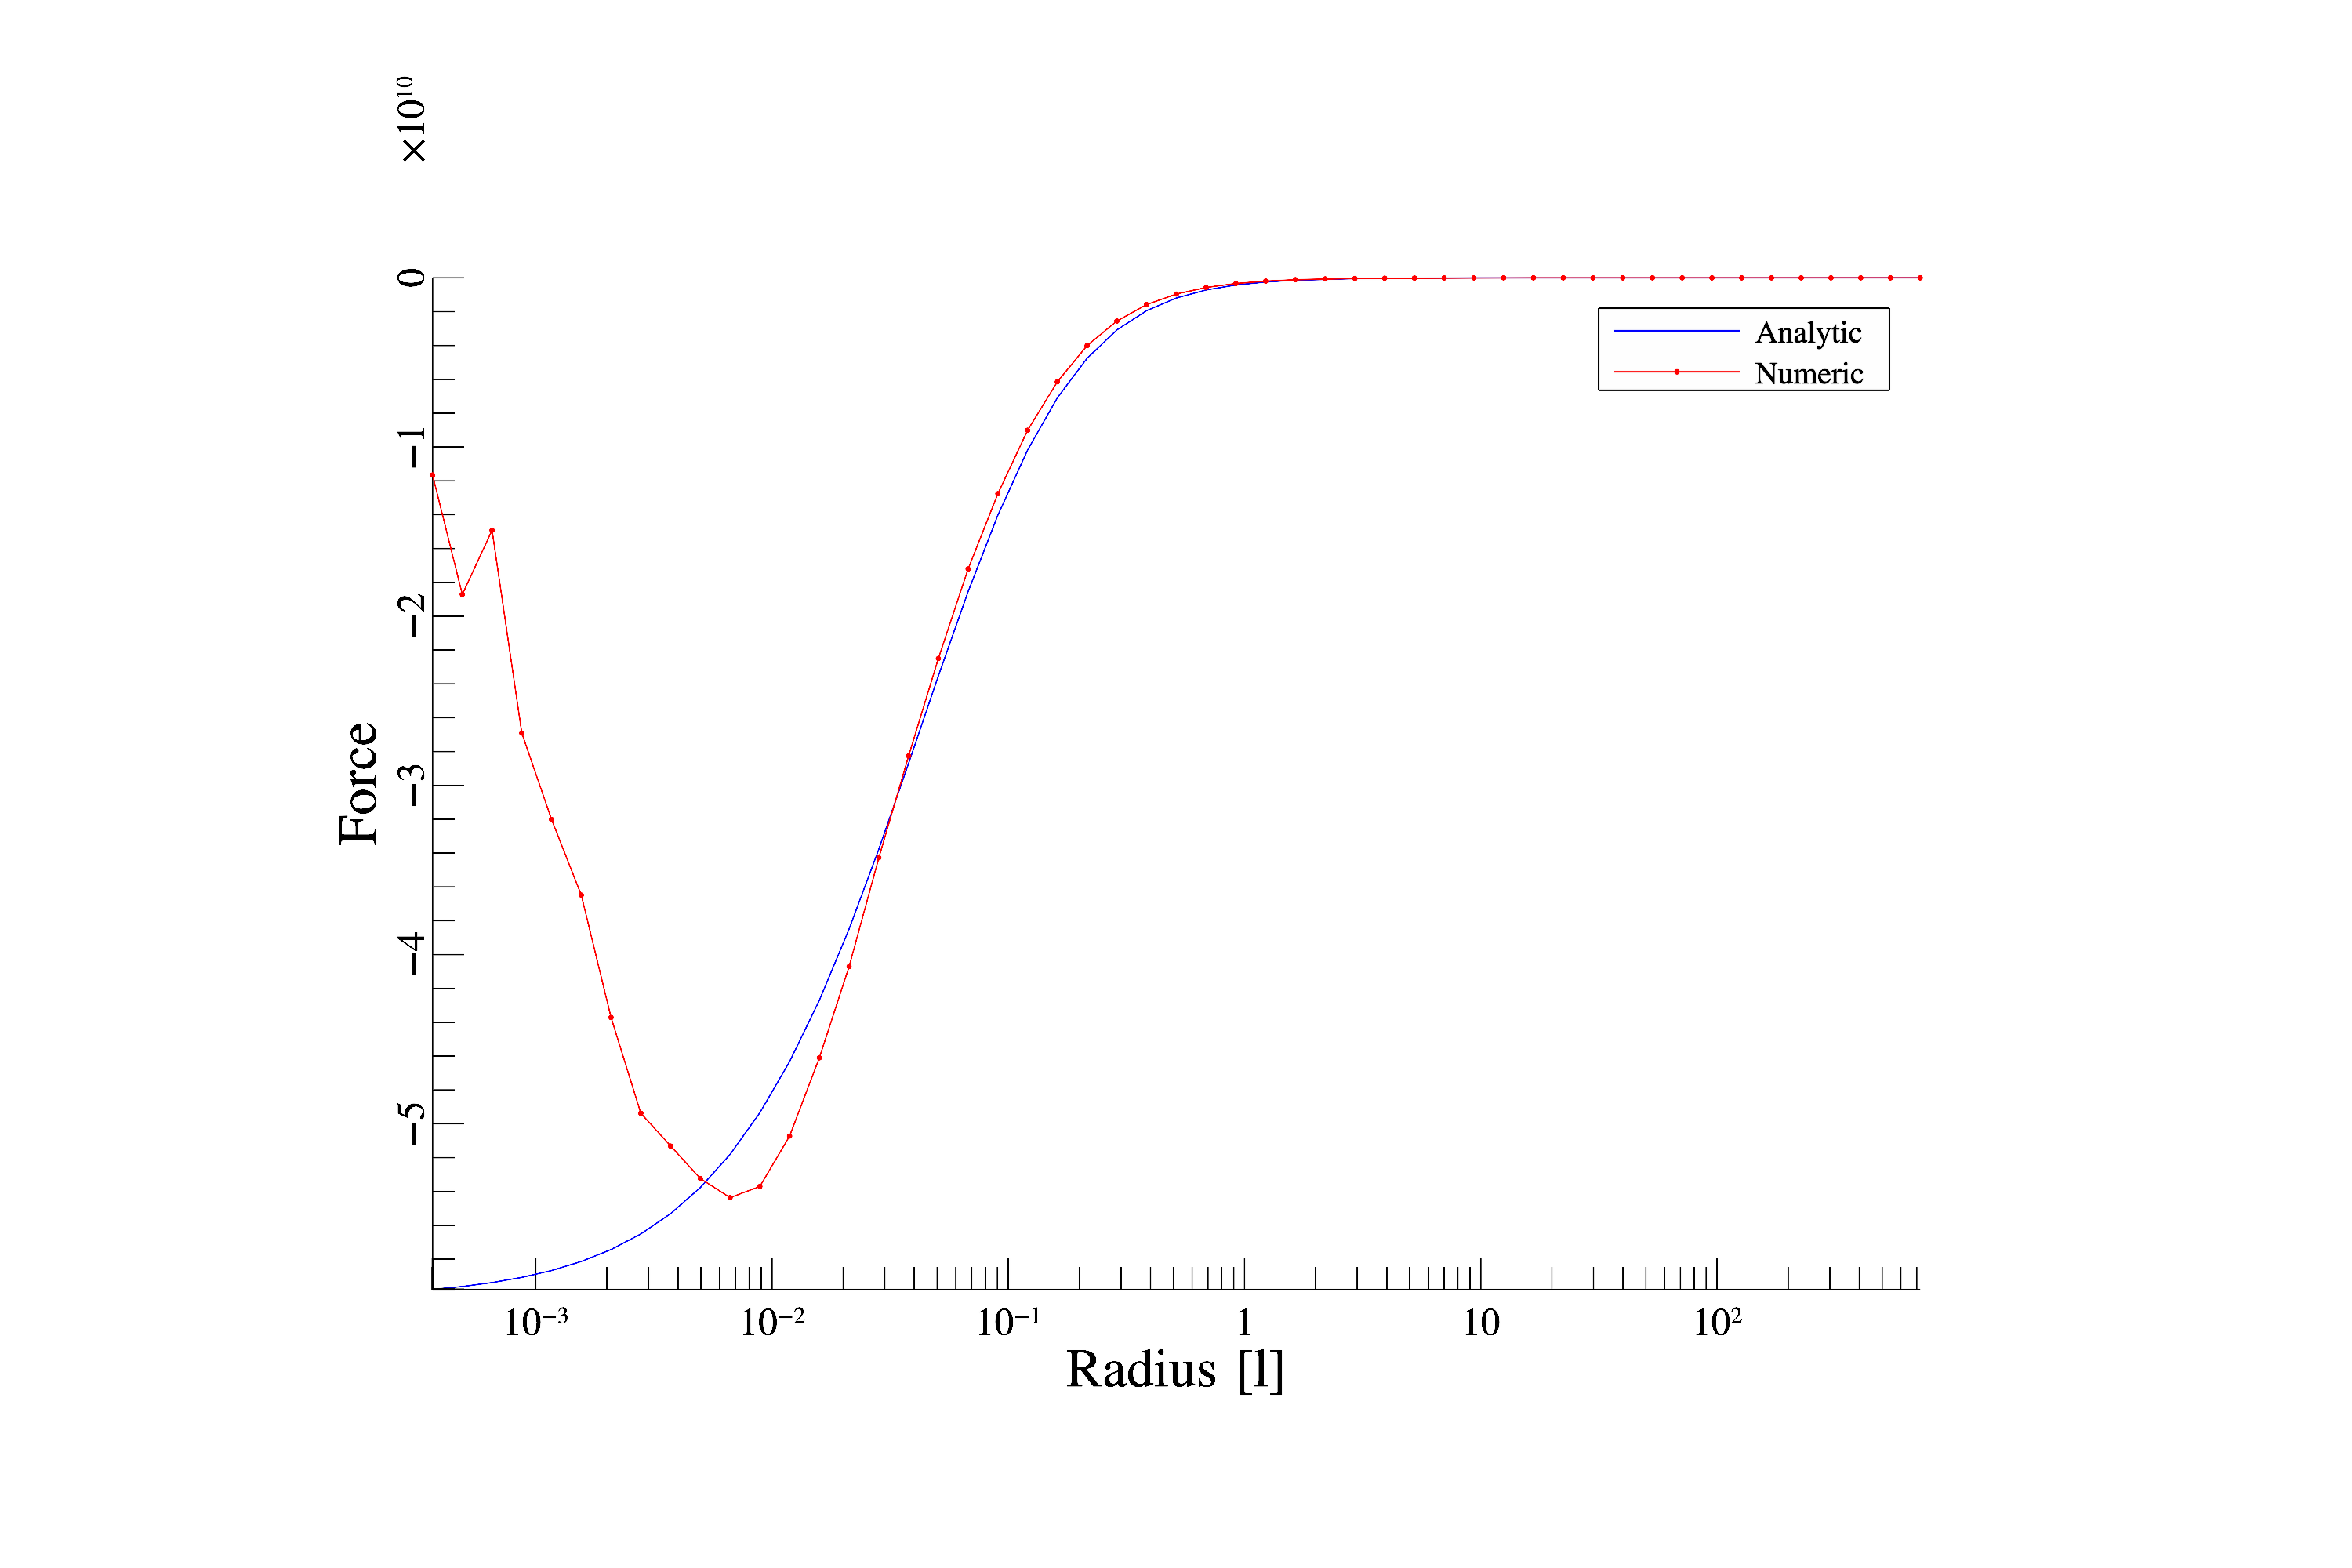
\includegraphics[width=0.95\textwidth]{figures/plots/forces_1.png}
\end{frame}

\begin{frame}{Softening /= 8}
	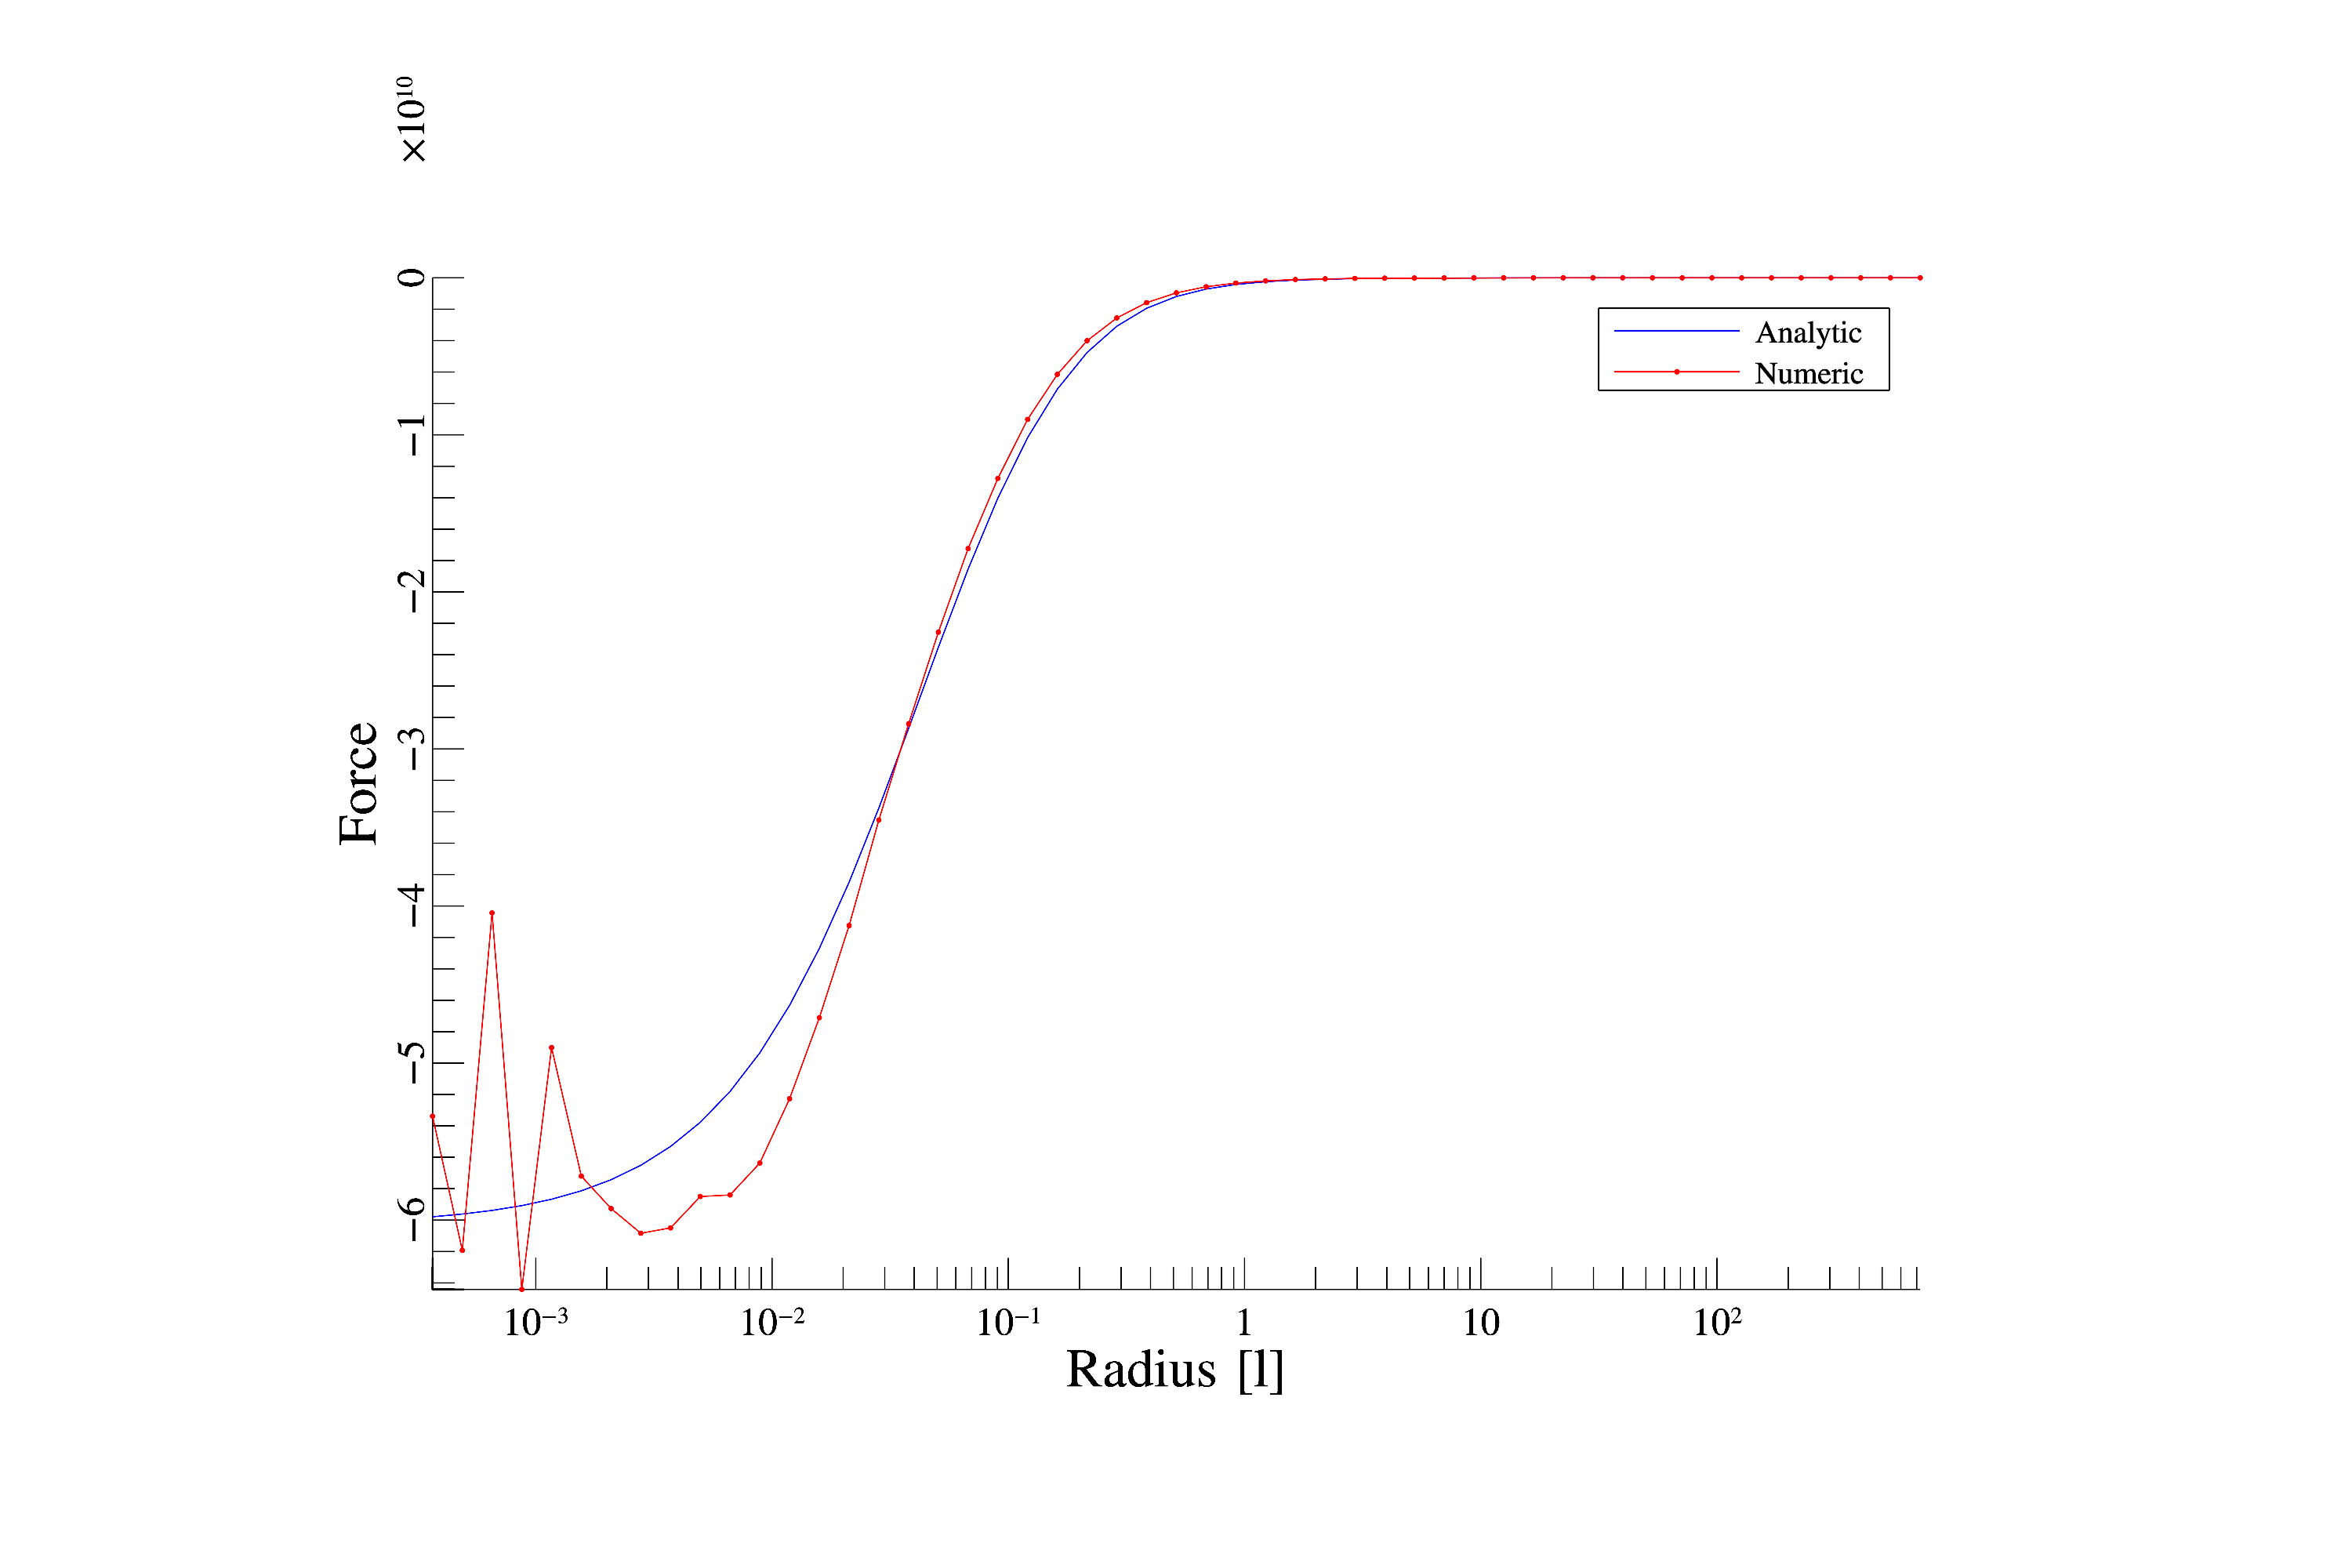
\includegraphics[width=0.95\textwidth]{figures/plots/forces_8.png}
\end{frame}

\begin{frame}{Softening /= 16}
	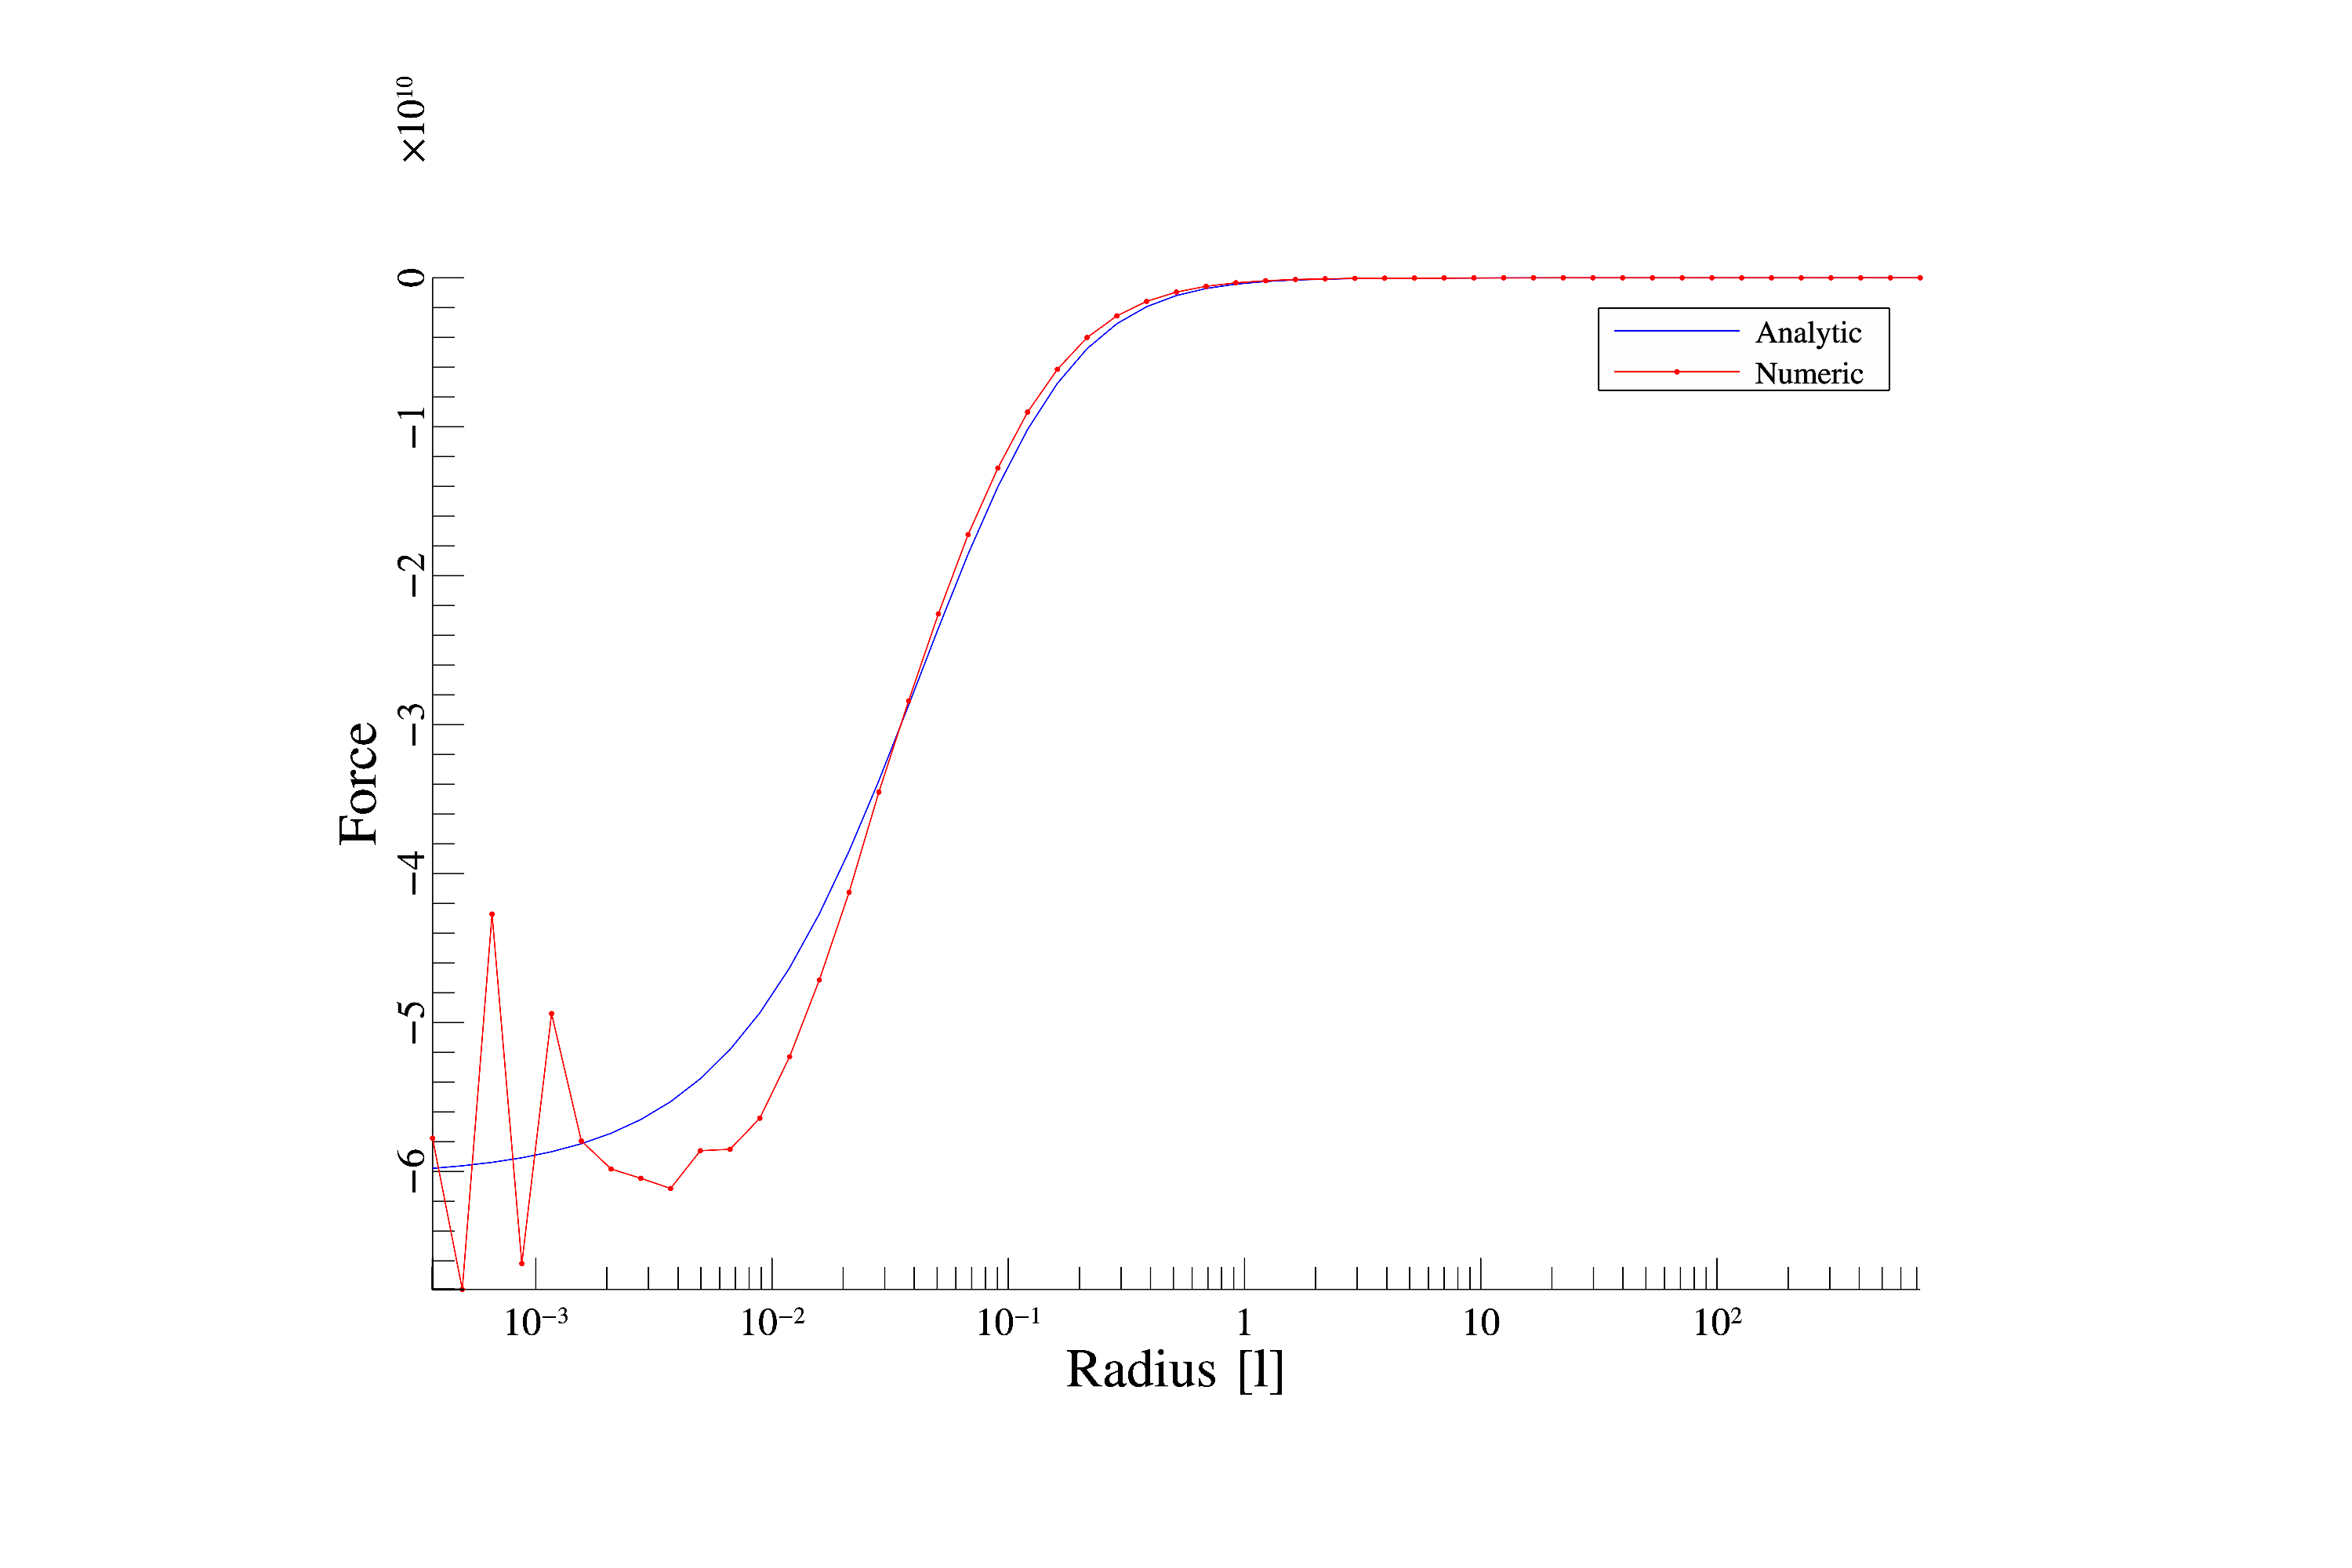
\includegraphics[width=0.95\textwidth]{figures/plots/forces_16.png}
\end{frame}

\begin{frame}{Softening /= 32}
	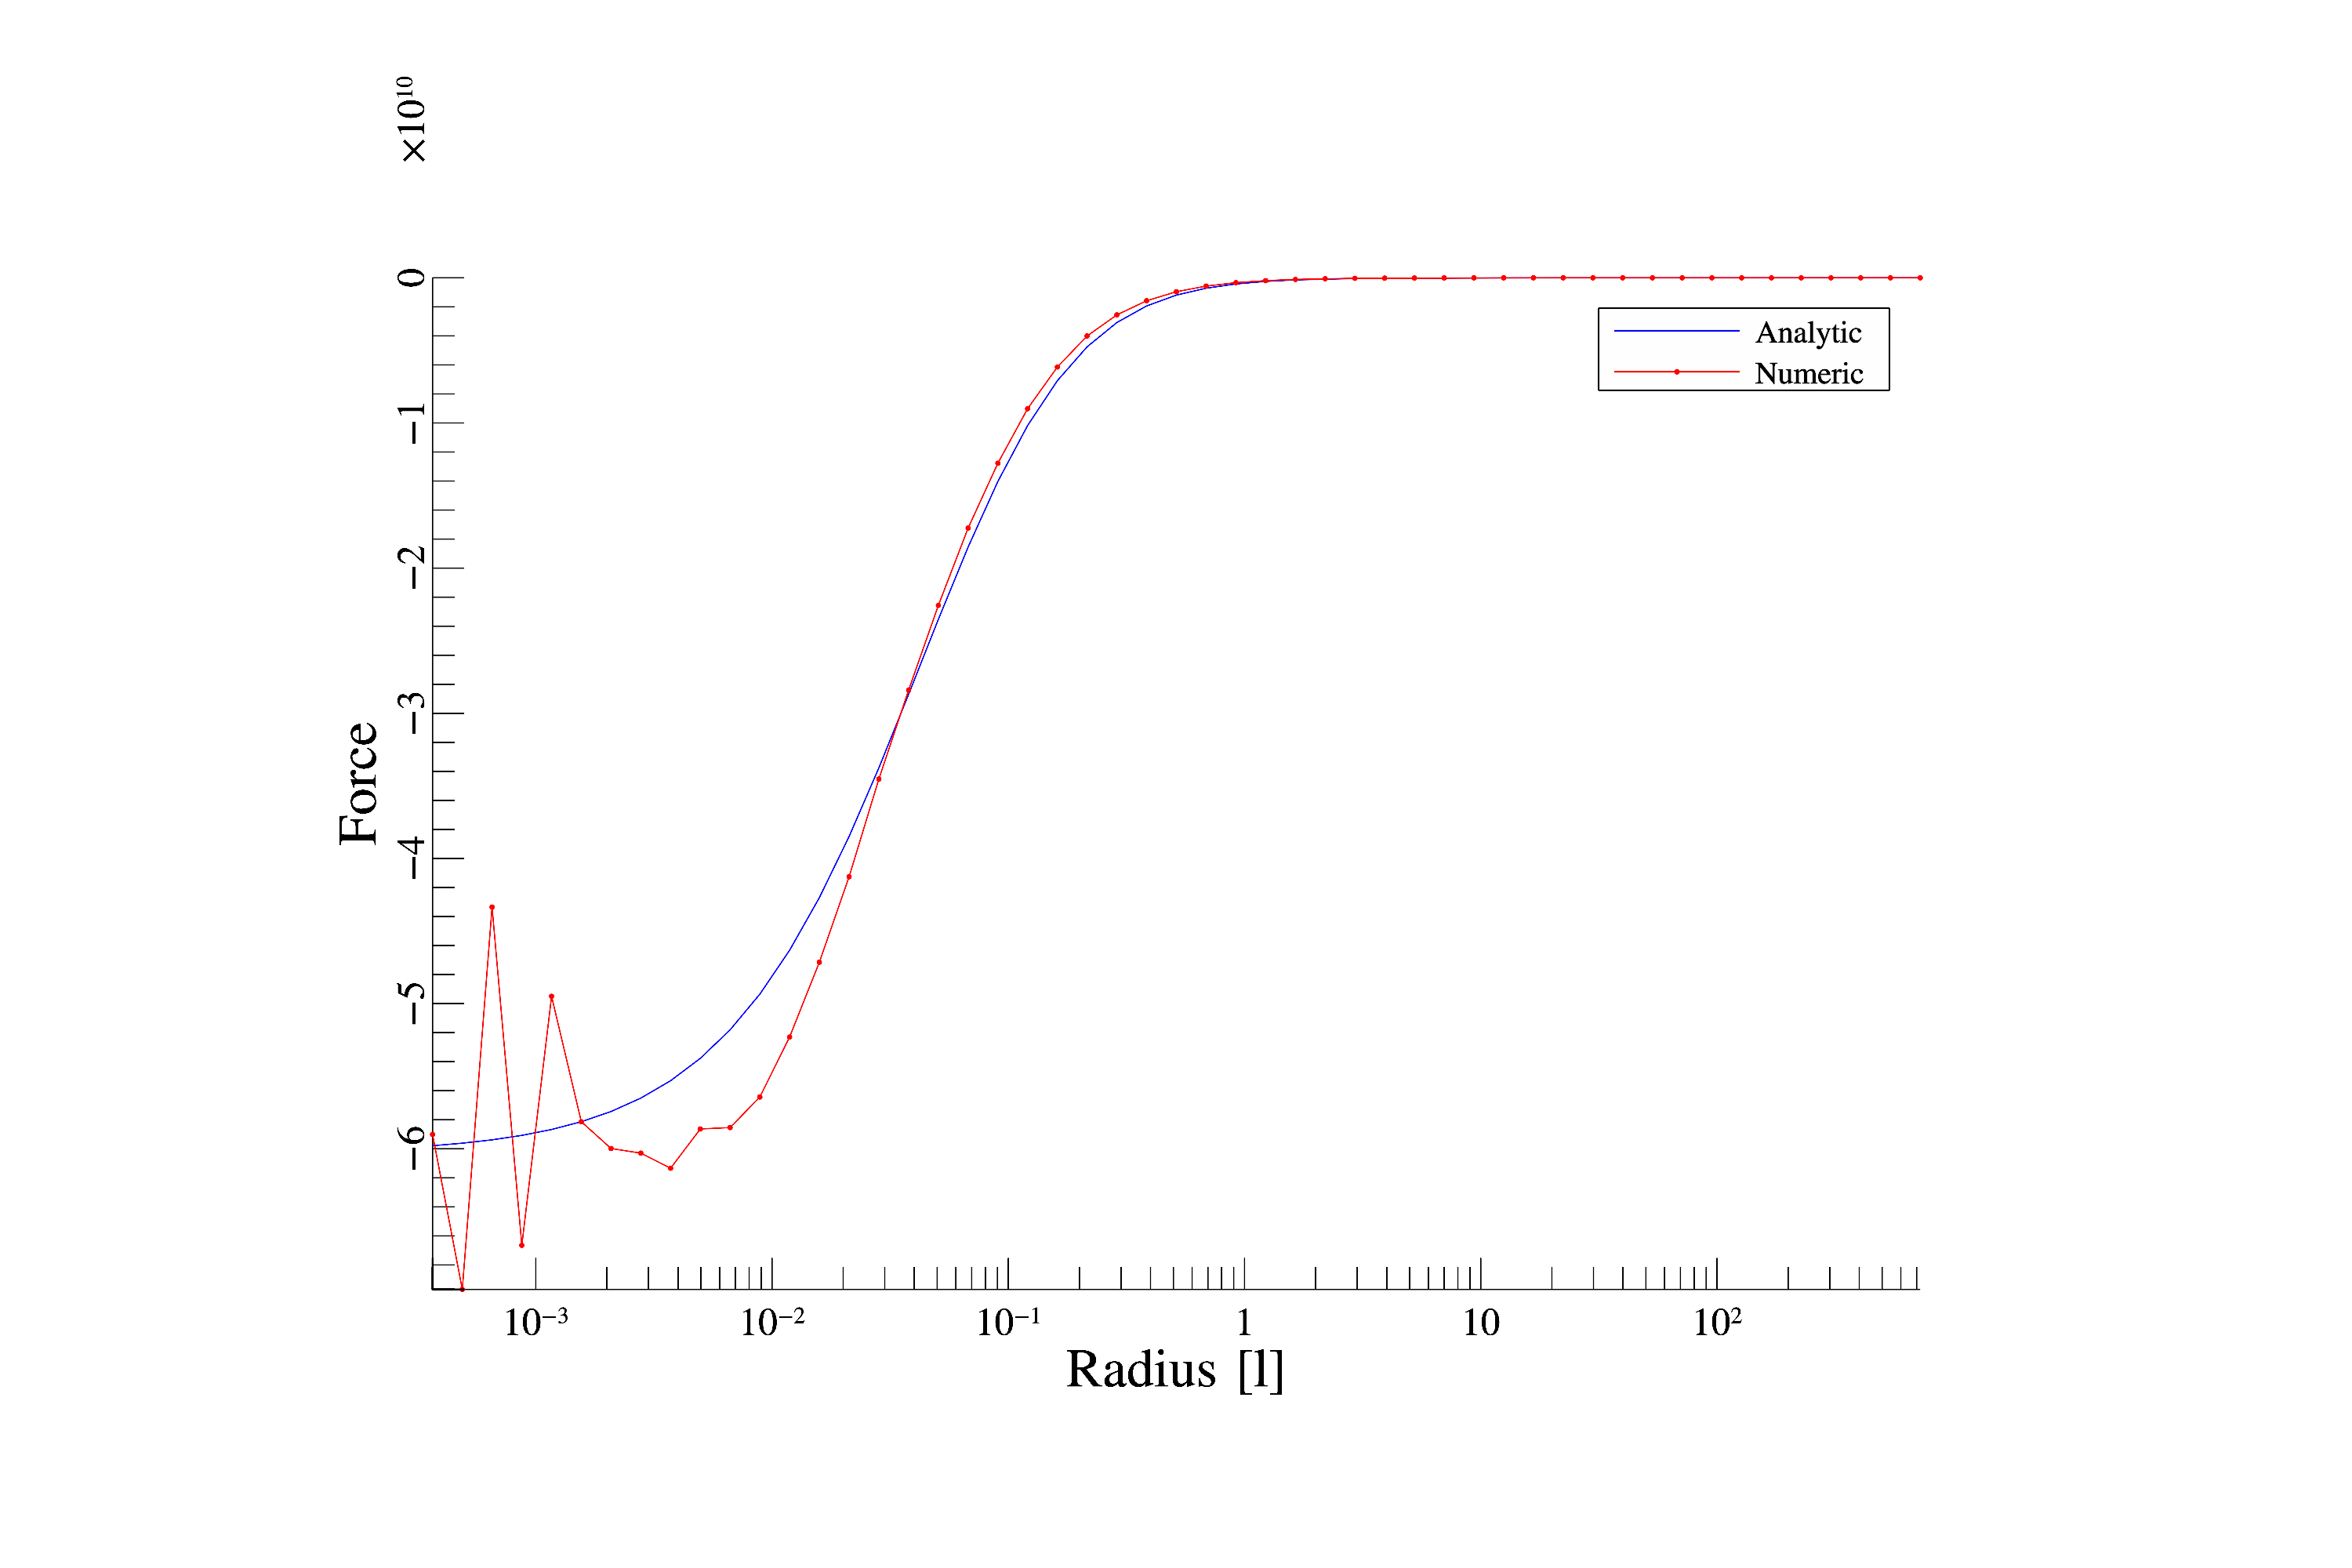
\includegraphics[width=0.95\textwidth]{figures/plots/forces_32.png}
\end{frame}

\begin{frame}{Softening /= 64}
	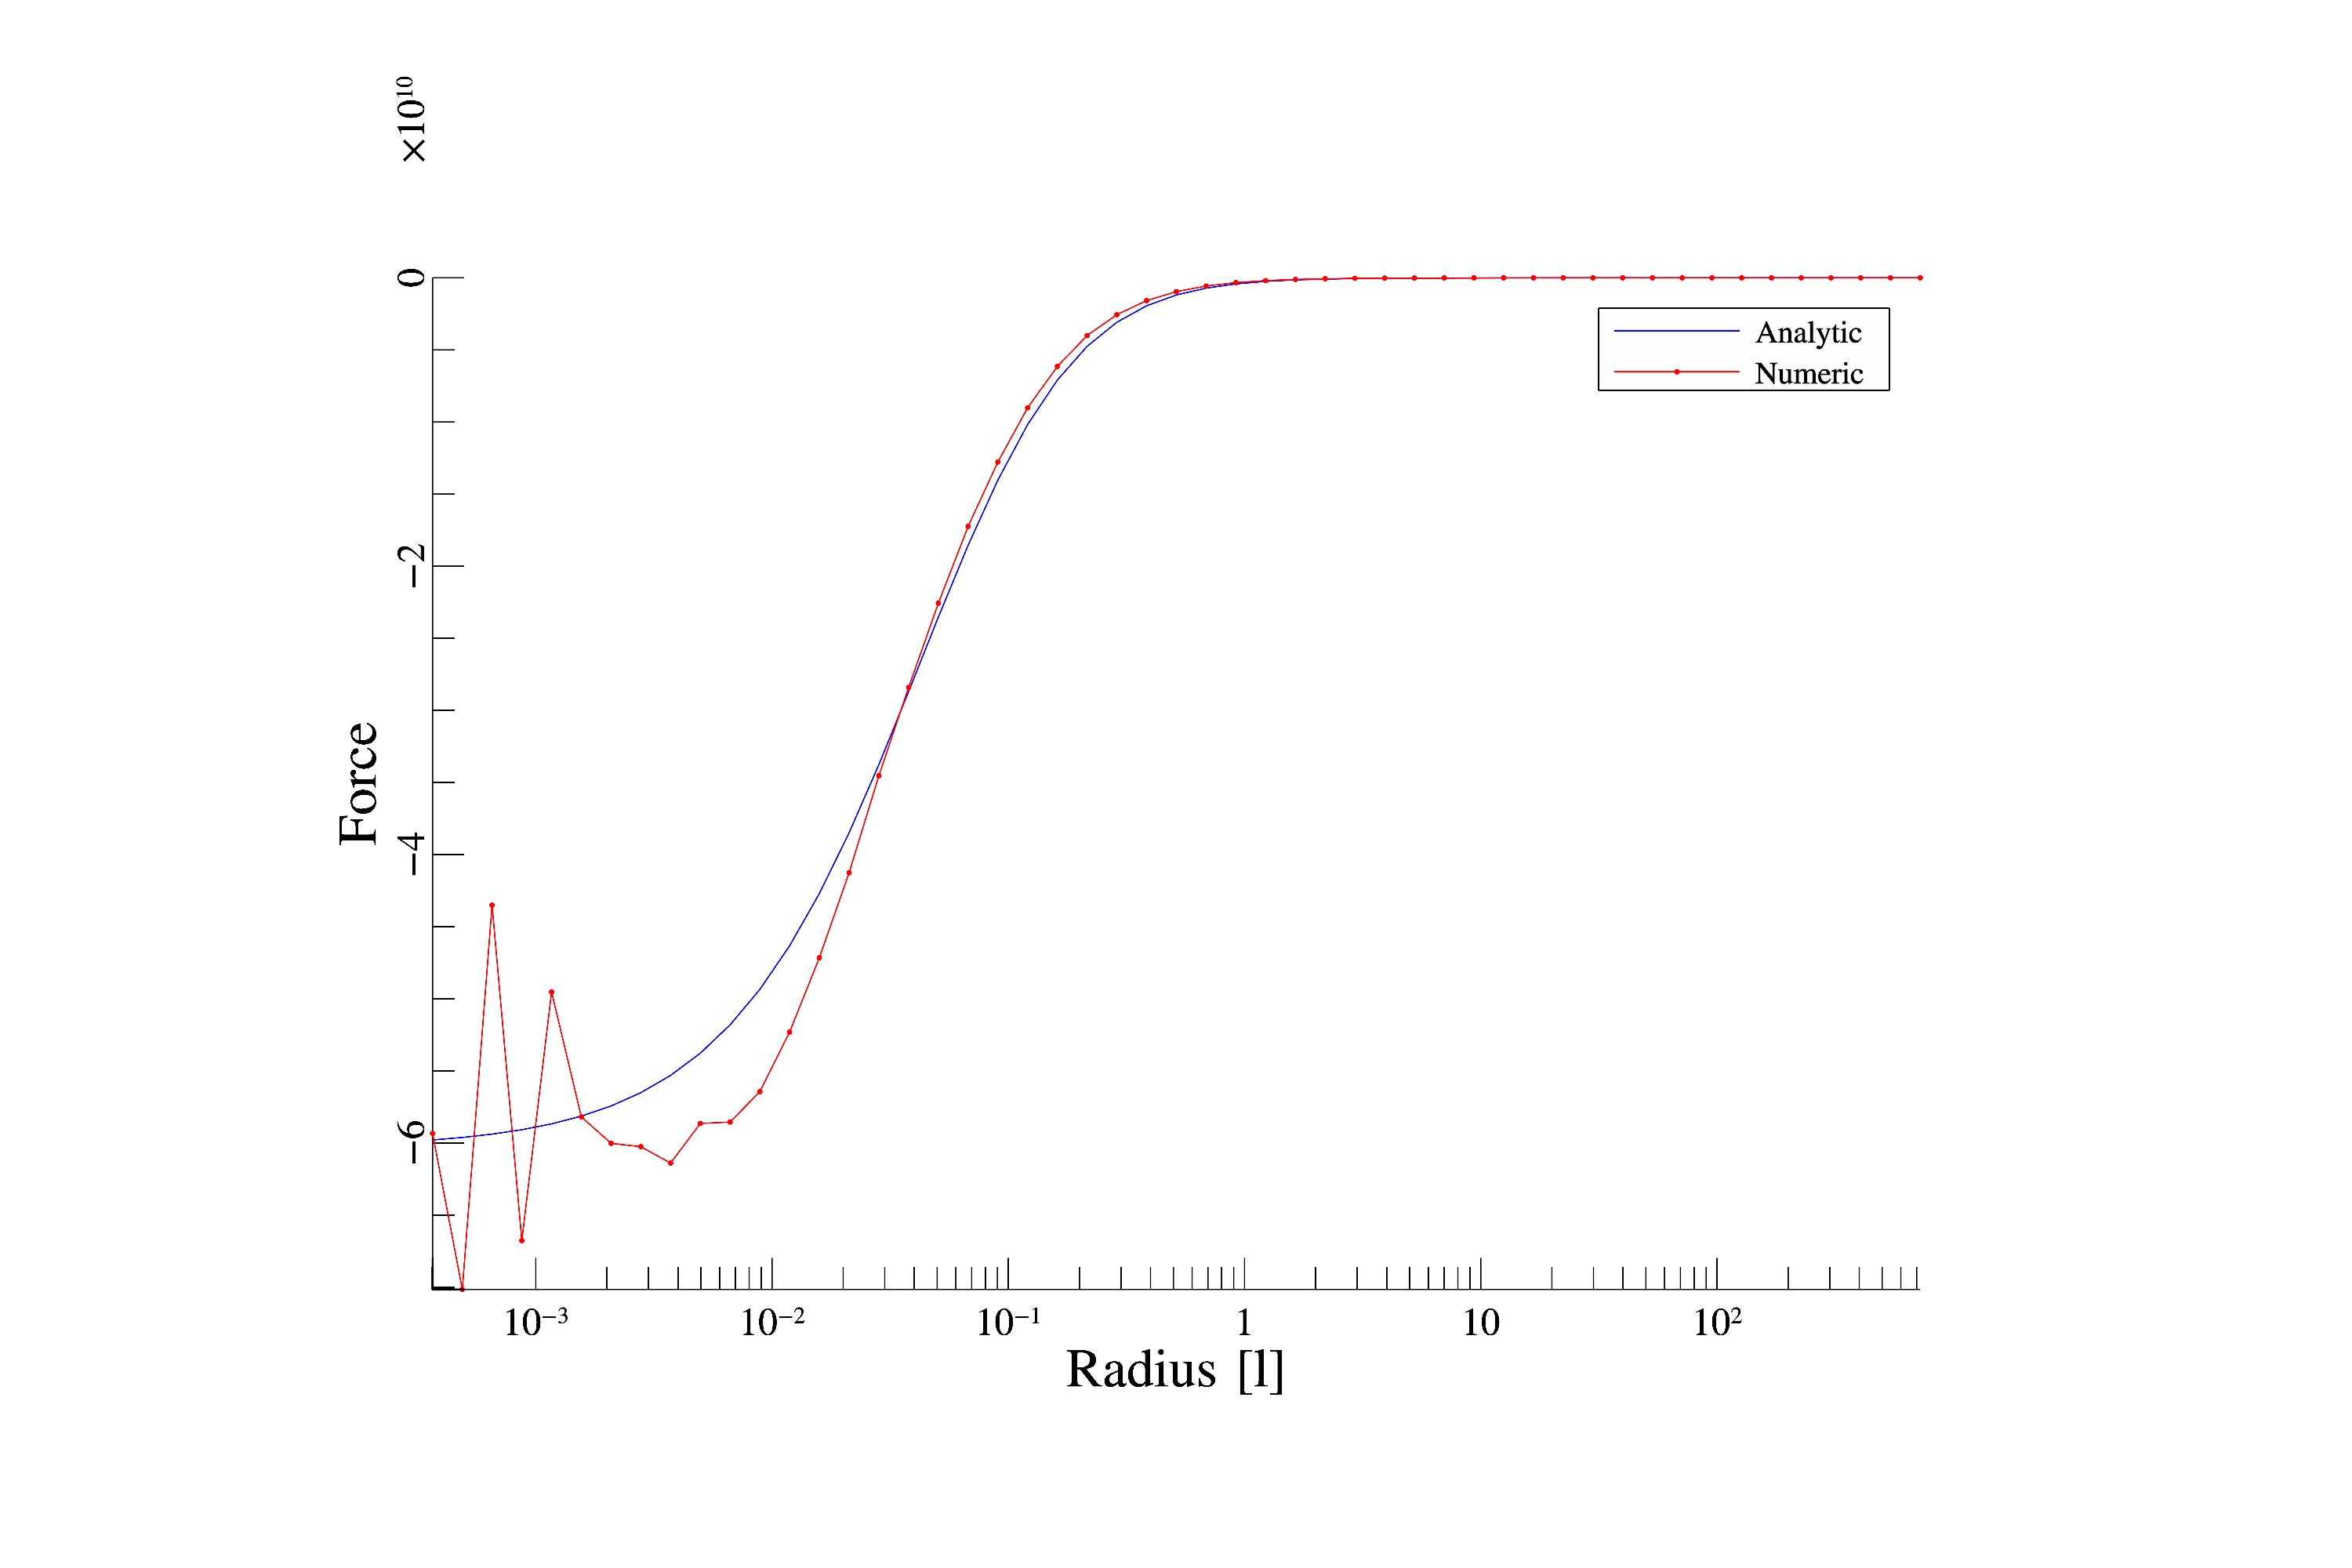
\includegraphics[width=0.95\textwidth]{figures/plots/forces_64.png}
\end{frame}

\begin{frame}{Softening /= 128}
	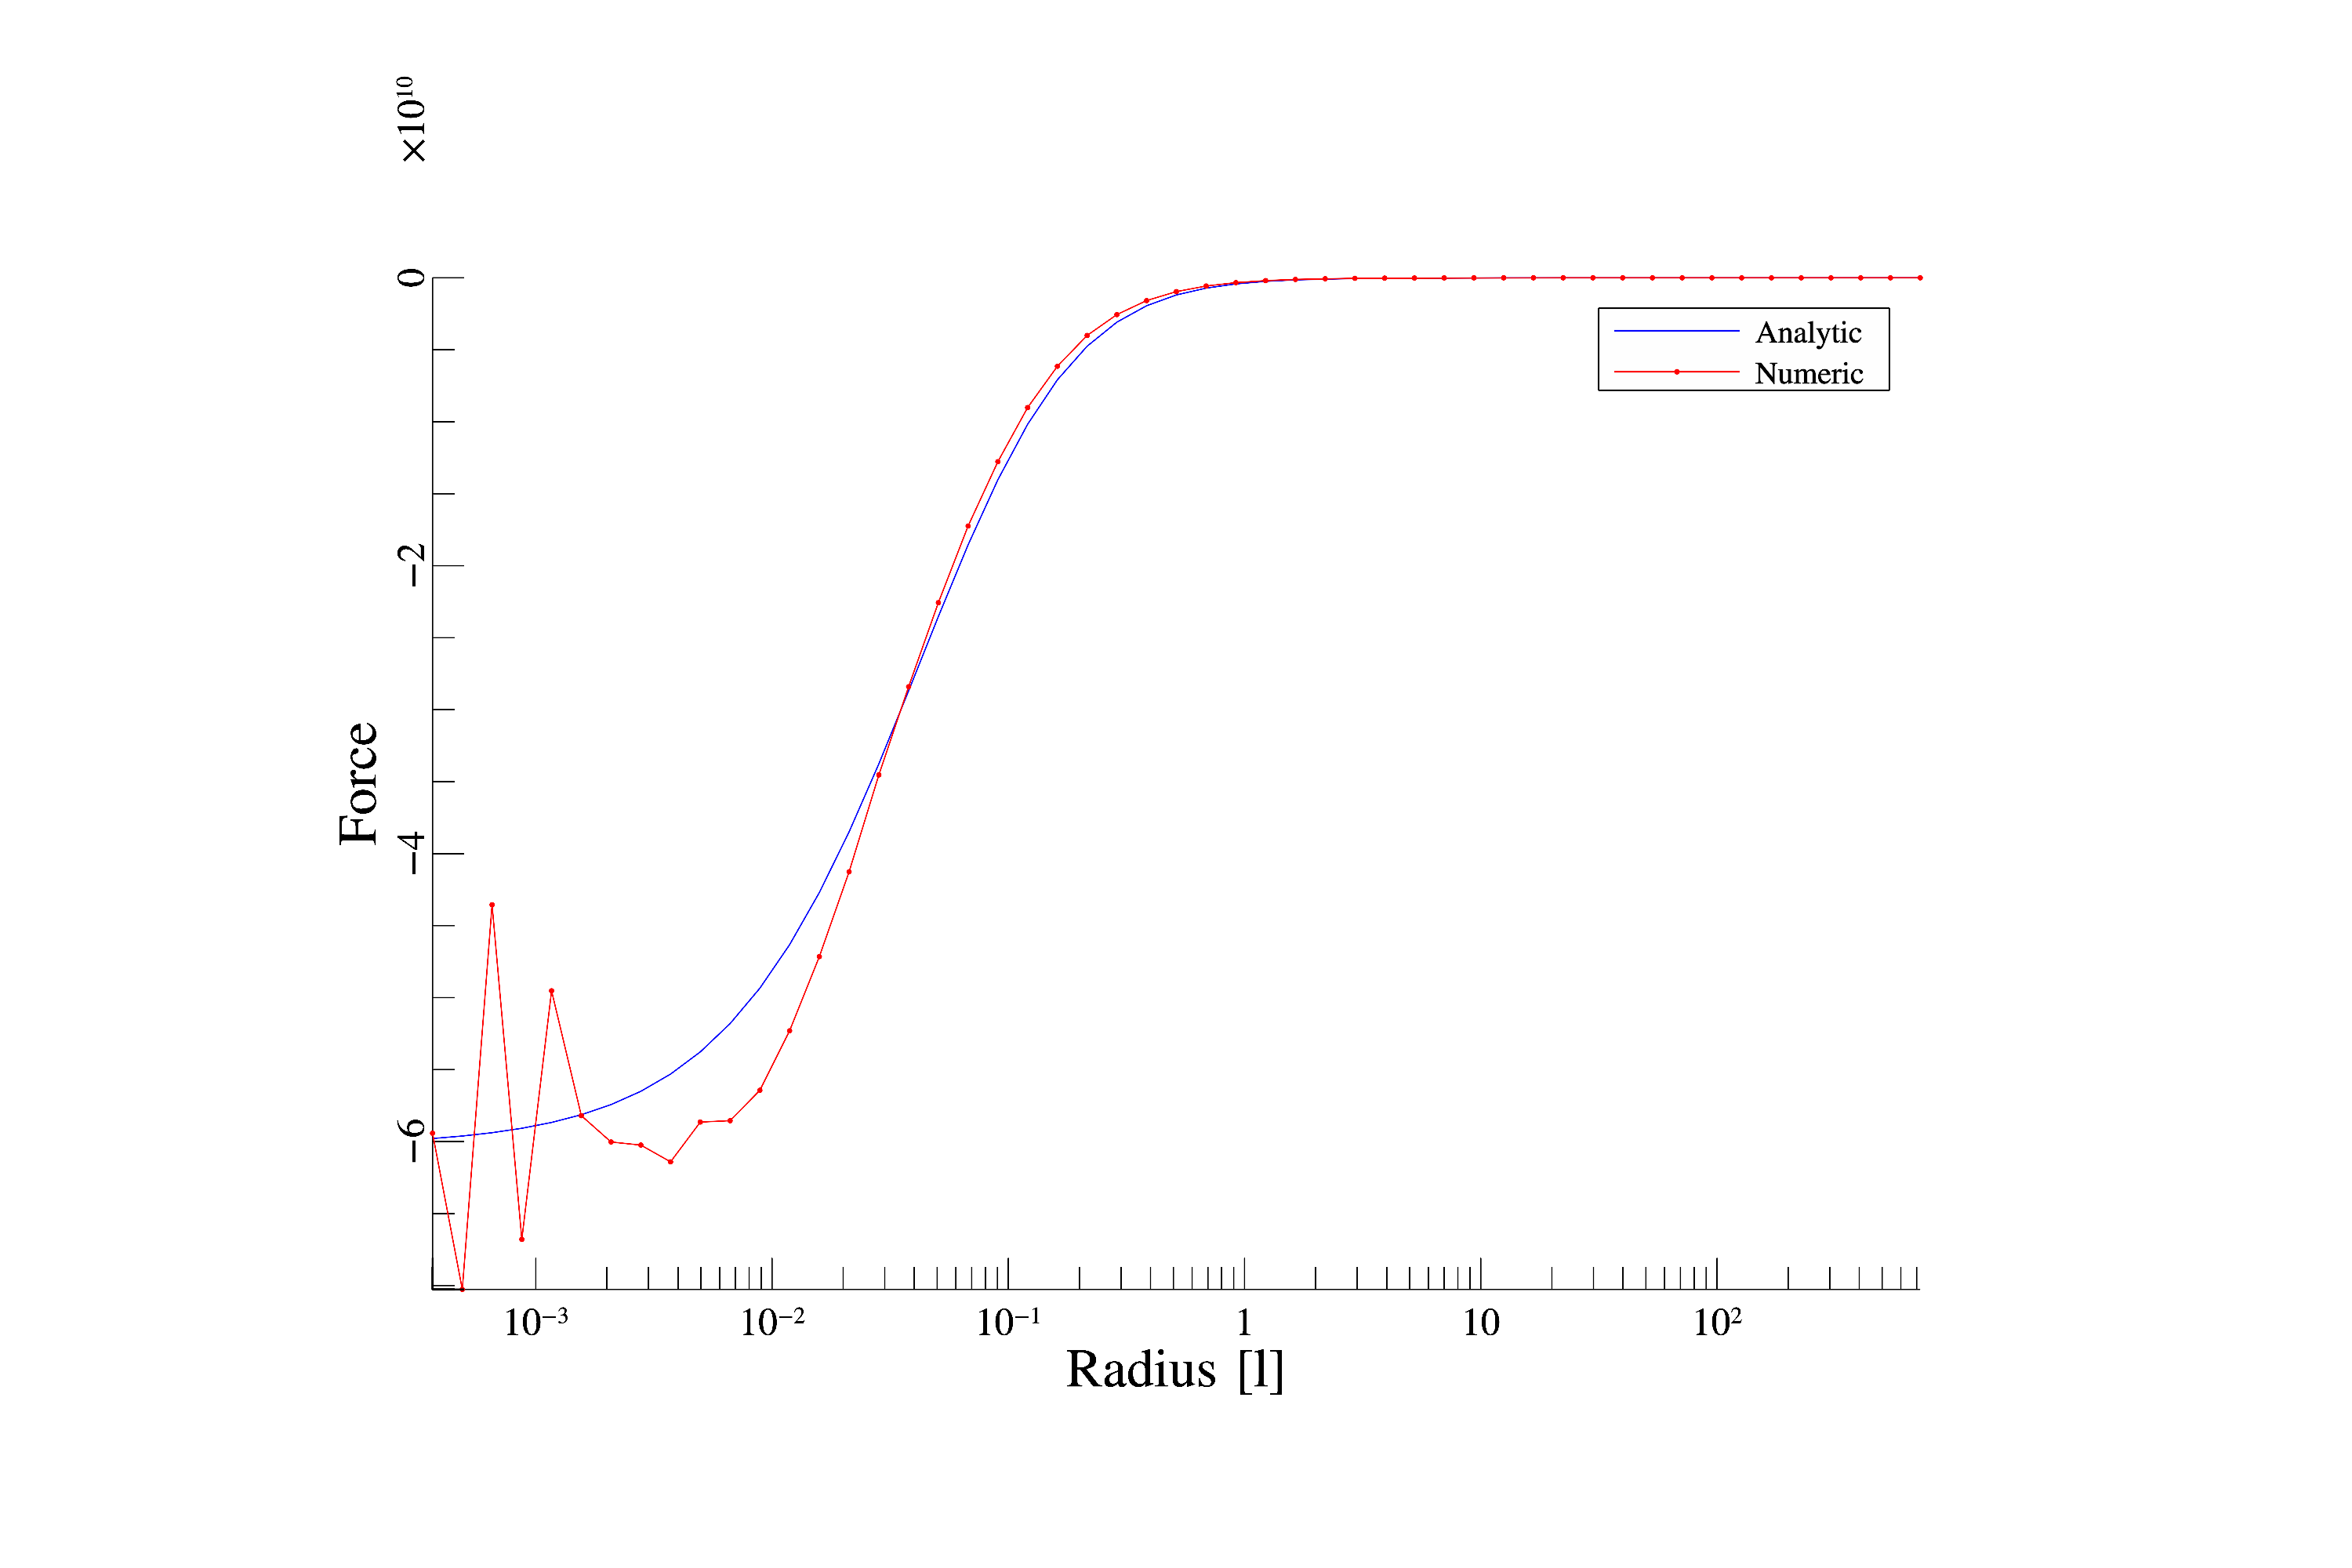
\includegraphics[width=0.95\textwidth]{figures/plots/forces_128.png}
\end{frame}

\begin{frame}{Relaxation Timescale}
	% Increasing the gravitational softening above the interparticle separation alters the close encounters between particles.
	% It reduces the impact of these encounters on particle trajectories.
	% As a result, the energy exchange during encounters becomes less efficient. This would typically lead to an 
	% increase in the relaxation timescale, because it would take longer for the system to reach equilibrium due to
	% the less frequent and less effective energy exchanges.

	% Although, since the relaxation calculation is purely analytical, there is no real correlation between the
	% values.

	\begin{equation}
		v_c = \sqrt{GM(R_{hm})/R_{hm}}
		\label{eq:circular-velocity}
	\end{equation}
	\begin{equation}
		t_{cross} = \frac{R_{hm}}{v_c}
		\label{eq:crossing_timescale}
	\end{equation}
	\begin{equation}
		t_{relax} = \frac{N}{8\ln{N}}t_{cross}
		\label{eq:relaxation_timescale}
	\end{equation}

	\bigskip

	Using $G = \SI{4.3009172706e-3}{\parsec.\solarmass^{-1}.(\kilo\metre\per\second)^2}$ and $m = \SI{92.4259}{\solarmass}$: \\

	Crossing Timescale: $898.302\ yr$ \\
	Relaxation Timescale: $0.520\ Myr$

\end{frame}


\section{Task 2: Tree-Code}
\begin{frame}[plain]
	\huge{Tree-Code - Multipole Expansion}
\end{frame}

\subsection{Multipole Expansion}
\begin{frame}{Hierarchical Grouping}
	\begin{columns}
		\column{.35\linewidth}
		\begin{itemize}
			\item Octree
			\item Axis-aligned cubes
			\item Every particle is a leaf node
			\item Empty cubes not stored
			\item Children have $c^\prime = \frac{1}{2}c$ side length
		\end{itemize}
		\column{.65\linewidth}
		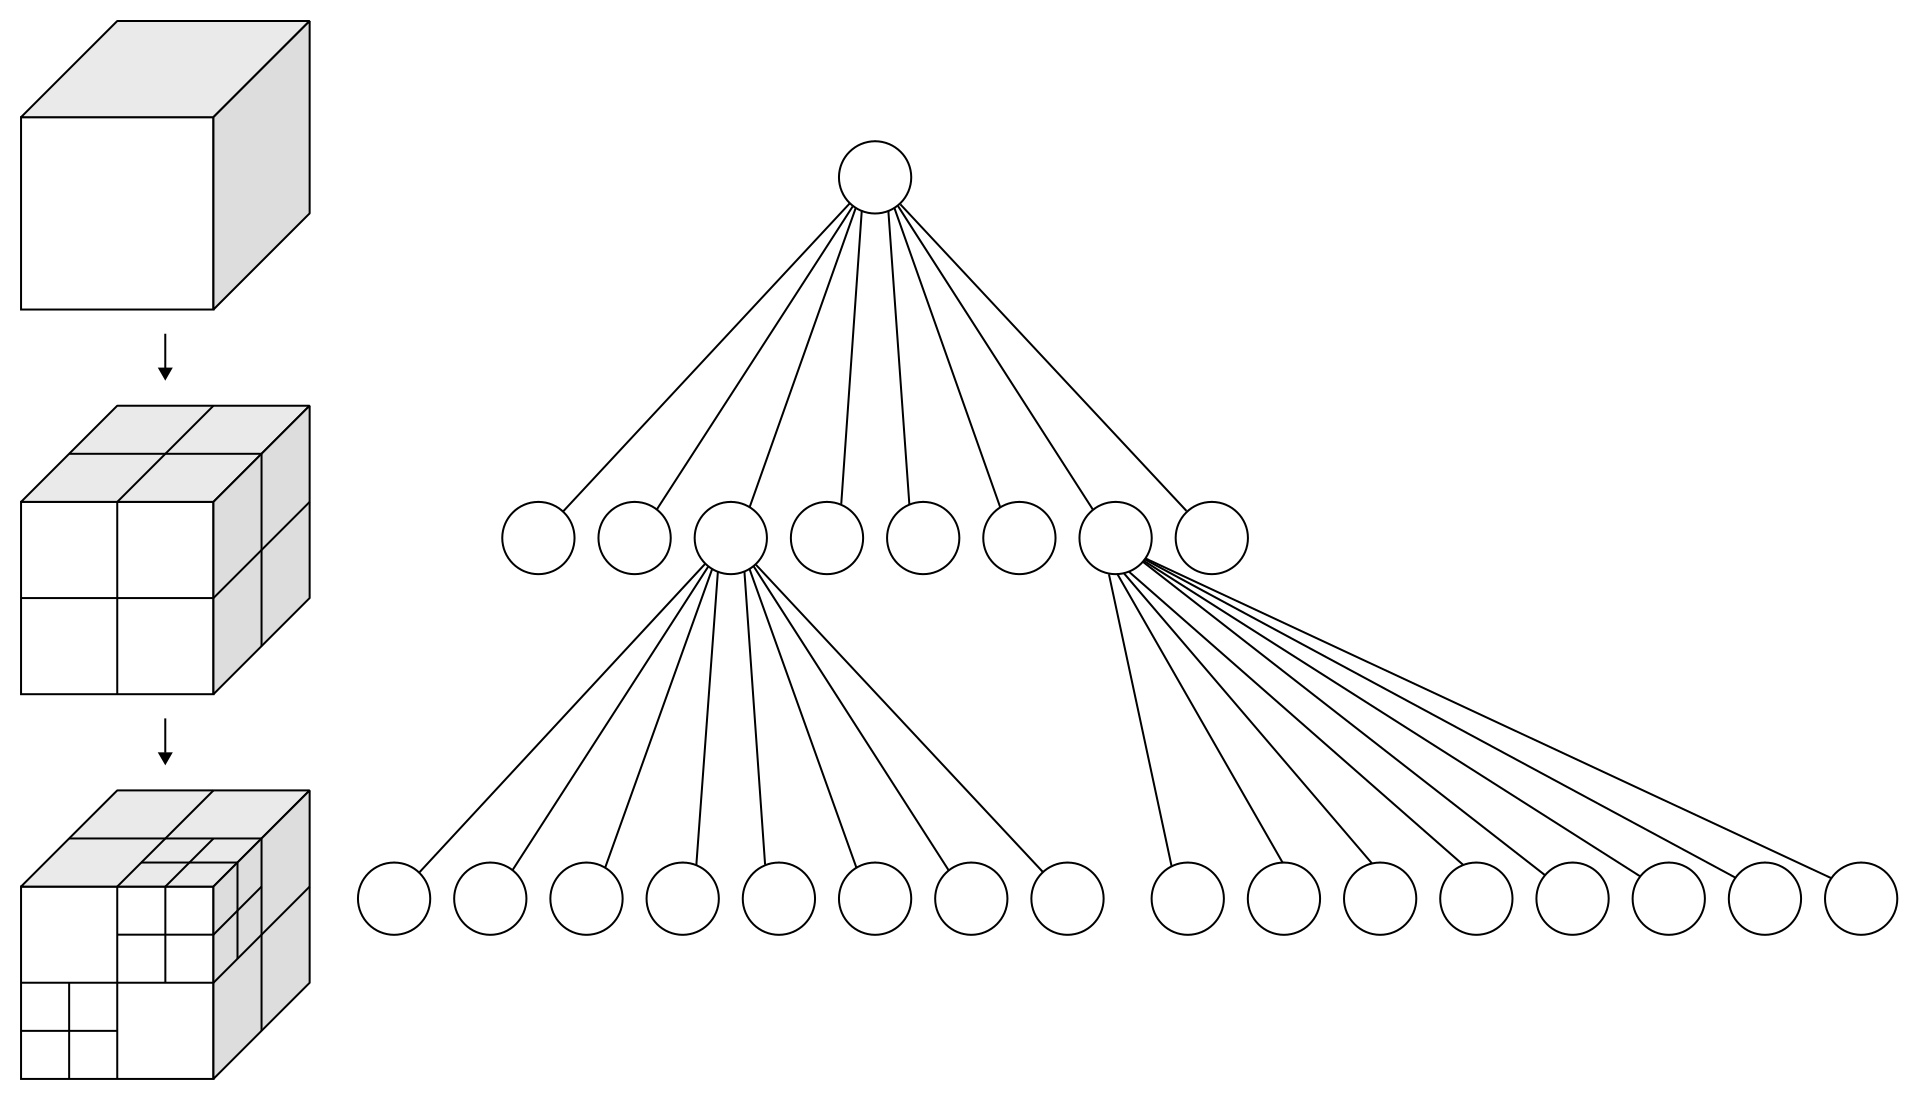
\includegraphics[width=\linewidth]{figures/cube.png}
	\end{columns}
\end{frame}

\begin{frame}[plain]{Octree}
	\includegraphics[width=\textwidth]{figures/plots/treecode.png}
\end{frame}

\begin{frame}{Multipole Expansion}
	\begin{columns}
		\column{.5\linewidth}
		\begin{itemize}
			\item $\vb{r}$ is sufficiently far
			      away
			\item  Seen under small opening angle
			      $\theta$
			\item  Orders of multipole corrections
		\end{itemize}
		\column{.5\linewidth}
		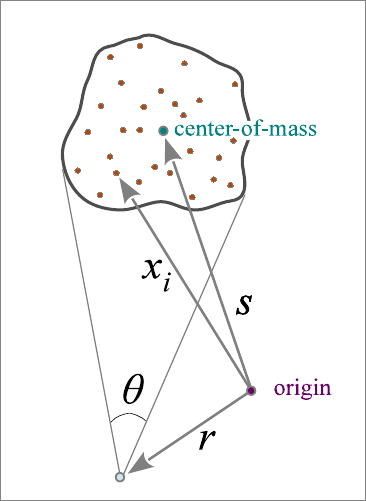
\includegraphics[width=\linewidth]{figures/multipole.png}
	\end{columns}
\end{frame}

\begin{frame}{Multipole Moments}
	\begin{itemize}
		\item Monopole
		      \begin{equation}
			      M = \sum_i m_i
		      \end{equation}
		\item Center of Mass
		      \begin{equation}
			      \vb{s} = \frac{1}{M}\sum_im_i\vb{x_i}
		      \end{equation}
		\item Quadrupole, Tensor calculation ($\vb{Q} \in \mathbb{R}^{3\times3}$)
		      \begin{equation}
			      \vb{Q}_{i j}=\sum_k m_k\left[3\left(\mathbf{s}-\mathbf{x}_k\right)_i\left(\mathbf{s}-\mathbf{x}_k\right)_j-\delta_{i j}\left(\mathbf{s}-\mathbf{x}_k\right)^2\right]
		      \end{equation}
	\end{itemize}
\end{frame}

\begin{frame}{Gravitational Potential \& Force}
	\begin{itemize}
		\item Potential:
		      \begin{equation}
			      \Phi(\mathbf{r_i})=-G\left[\frac{M}{|\mathbf{y}|}+\frac{1}{2} \frac{\mathbf{y}^T \mathbf{Q} \mathbf{y}}{|\mathbf{y}|^5}\right], \quad \mathbf{y}=\mathbf{r}_i-\mathbf{s}
		      \end{equation}
		\item Monopole Force:
		      \begin{equation}
			      \vb{F}_M(\vb{r}_i) = -G \frac{m_i  M}{ | \vb{y} | ^3}\vb{y}
		      \end{equation}
		\item Quadrupole Force:
		      \begin{equation}
			      \vb{F}_Q(\vb{r}_i) = G\left[\frac{\vb{Q}\vb{y}}{ | \vb{y} | ^4} - \frac{5}{2}
				      \frac{\vb{y}^T \vb{Q} \vb{y}} { | \vb{y} | ^4} \vb{y}\right]
		      \end{equation}
		\item Total Force:
		      \begin{equation}
			      \vb{F}(\vb{r}_i) = \vb{F}_M + \vb{F}_Q
		      \end{equation}
	\end{itemize}
\end{frame}

\begin{frame}{When to apply the expansion?}
	\begin{itemize}
		\item Opening angle:
		      \begin{equation}
			      \theta \approx \frac{c}{|\vb{y}|}
		      \end{equation}
		\item Tolerance Angle $\theta_c \in [0.5, 1]$
		\item In the limit $\theta_c \rightarrow 0$  direct summation force.
	\end{itemize}\bigskip

	{\footnotesize
		Where:
		\begin{itemize}
			\item $c$ - Length of cube side
			\item $\vb{y}$ - Vector: particle position to center of mass
		\end{itemize}
	}
\end{frame}

\begin{frame}{Tree Walk}
	\begin{itemize}
		\item Depth-First traversal
	\end{itemize}
	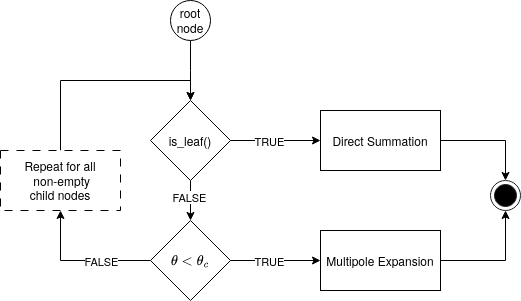
\includegraphics[width=0.95\textwidth]{figures/multipole_uml.png}
\end{frame}

\subsection{Direct Summation}
\begin{frame}{Integration with Direct Summation}
	$T = 5 \cross t_{cross}$ in dimensionless calculation with $\Delta t = \eta t_{cross}$. \bigskip

	Iteration on each particle with \texttt{OpenMP} and on each particle \textbf{Leapfrog} integration in \textit{kick-drift-kick} form:
	\begin{itemize}
		\item $v_{n+1/2} = r_0 + a_0  \frac{\Delta t}{2}$
		\item $r_{n+1} = r_0 + v_{n+1/2} \Delta t$
		\item $a_{n+1} = df(\Delta t)$
		\item $v_{n+1} = v_{n+1/2} + a_{n+1} \frac{\Delta t}{2}$
	\end{itemize} \bigskip

	{\footnotesize Where:
		\begin{itemize}
			\item $\eta = [0.1, 0.01]$
			\item $t_{cross} \approx 6e^{-6}$
			\item $df(\Delta t)$ - Direct force summation
		\end{itemize}
	}

	\bigskip\centering
	SHOW GIFS

\end{frame}

\begin{frame}{Force Comparison - Accuracy}
	Assumption: Direct Force summation considered most accurate. \\

	$\lim\limits_{\theta_c \to 0}$ leads to Direct Summation, often considered in the range of $[0.5, 1.0]$.
\end{frame}

\begin{frame}[allowframebreaks]{Force Comparison}
	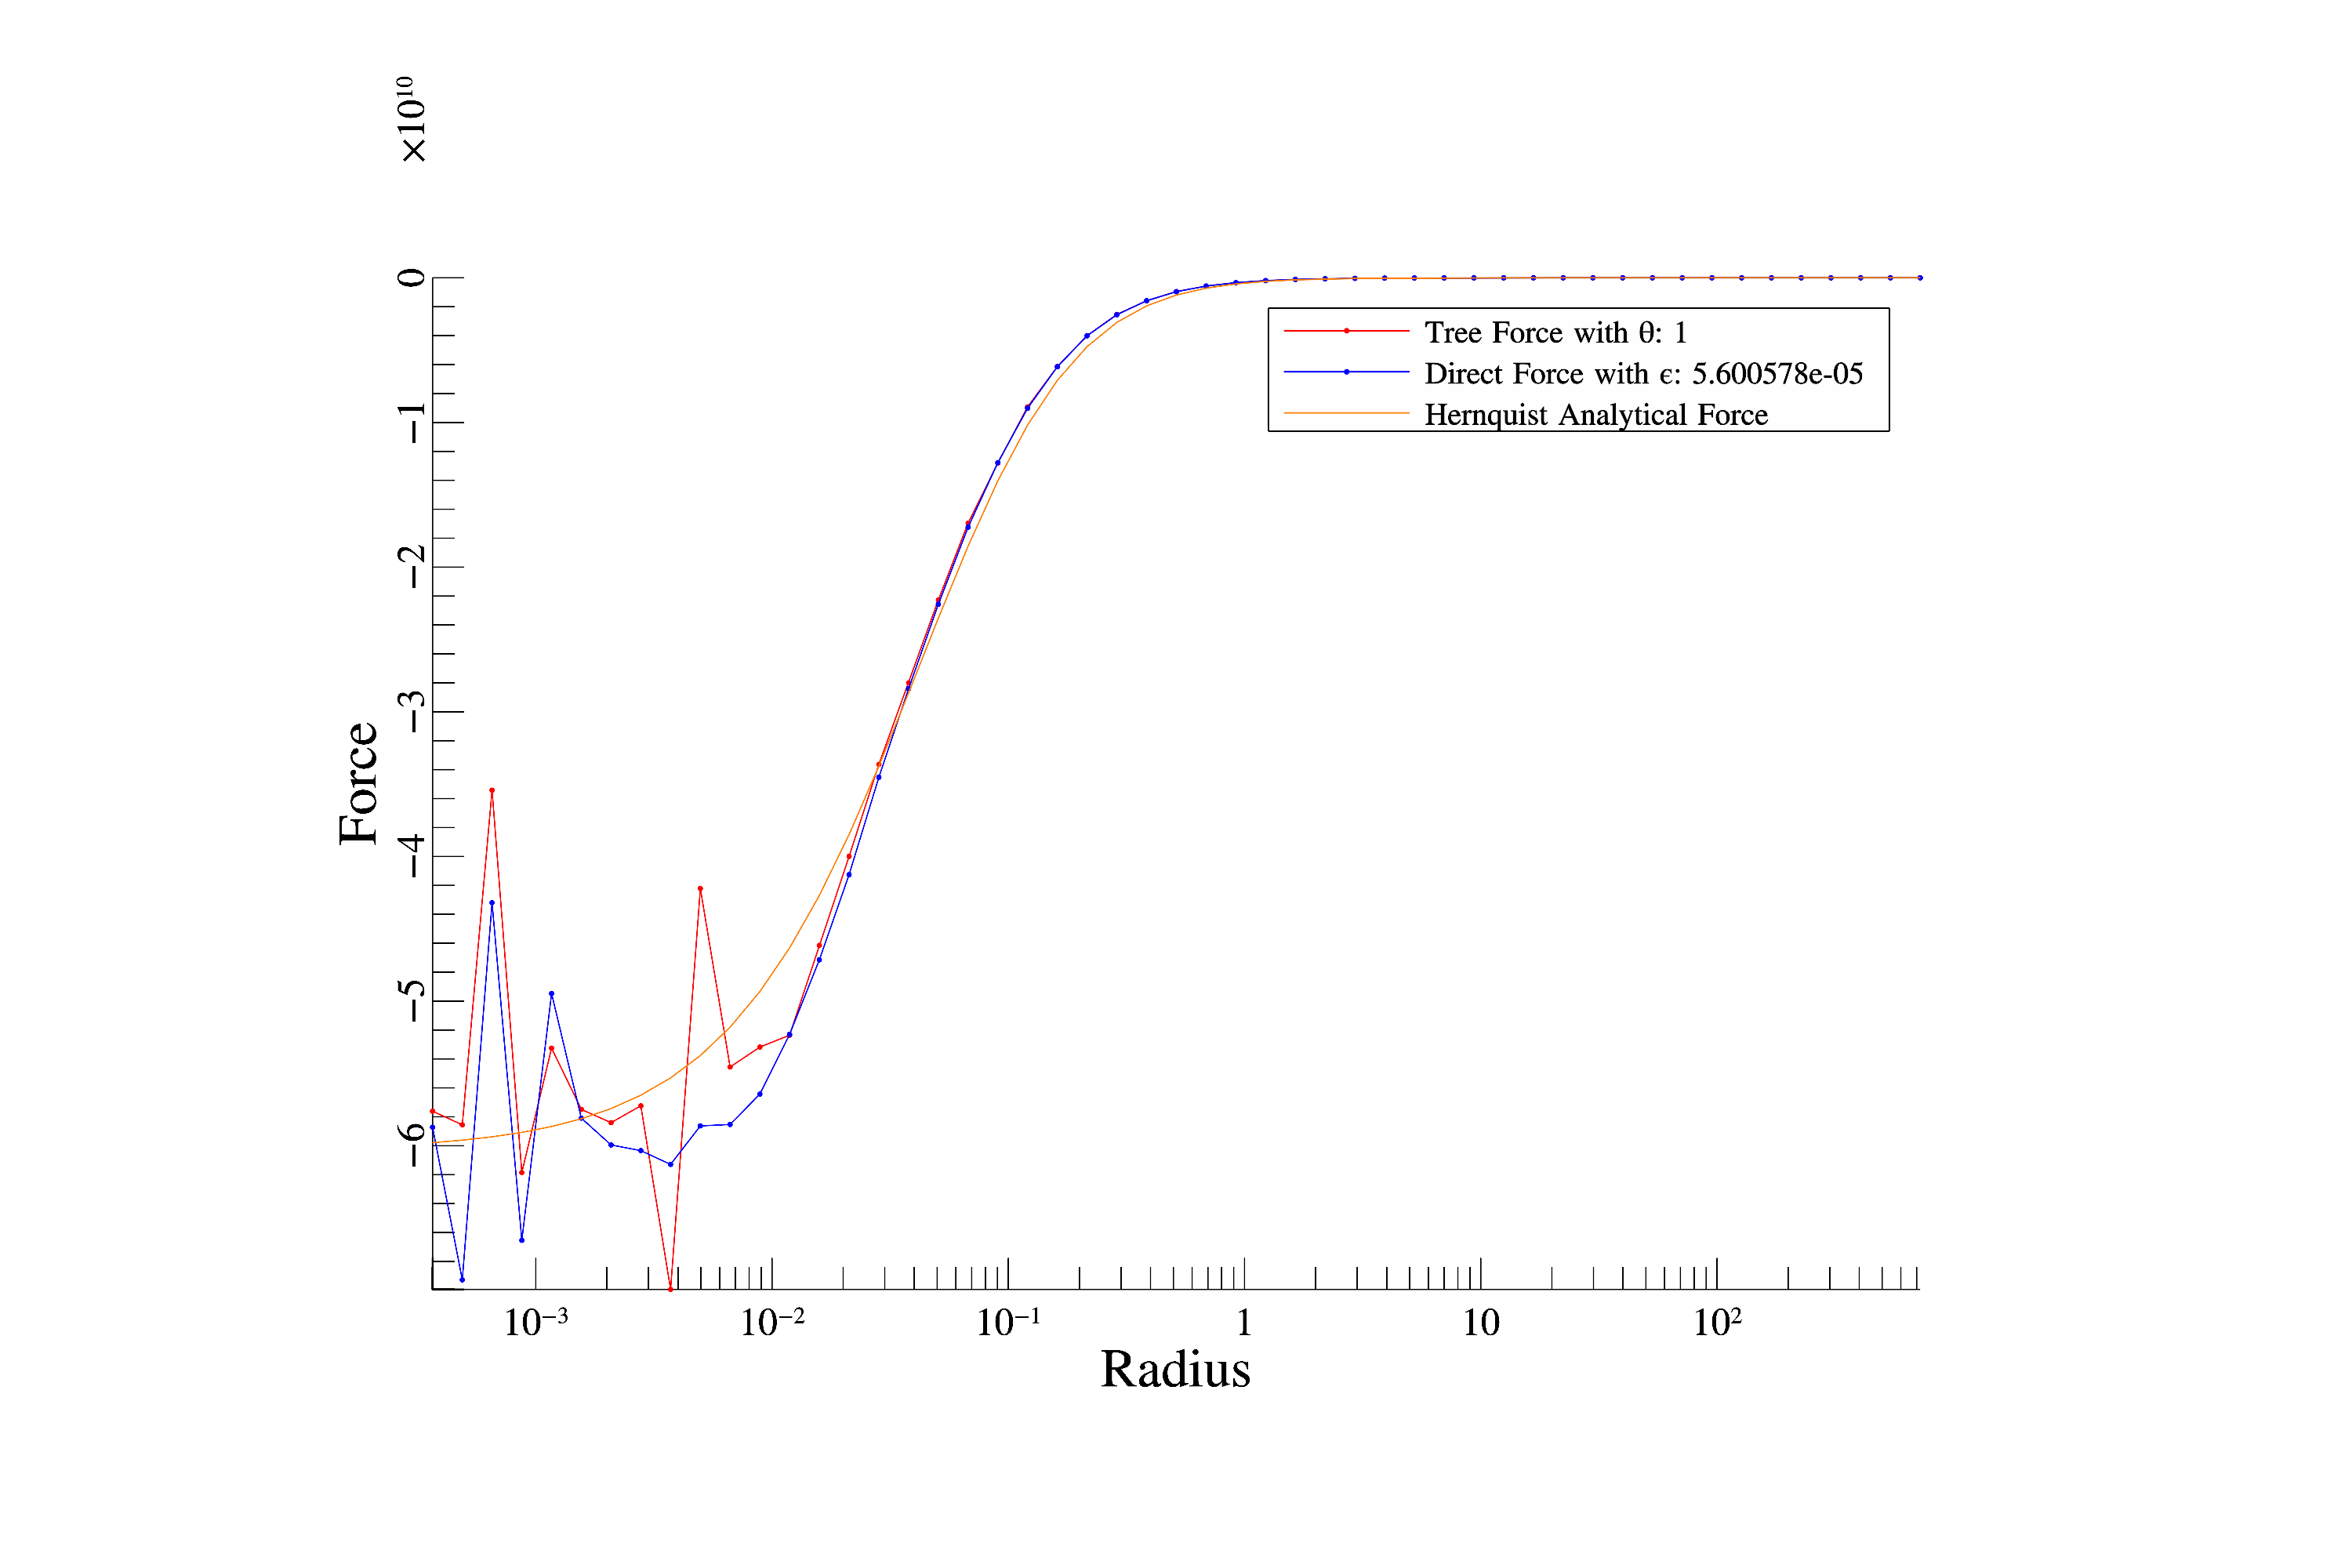
\includegraphics[width=\textwidth]{figures/plots/tree_force_1.png}
	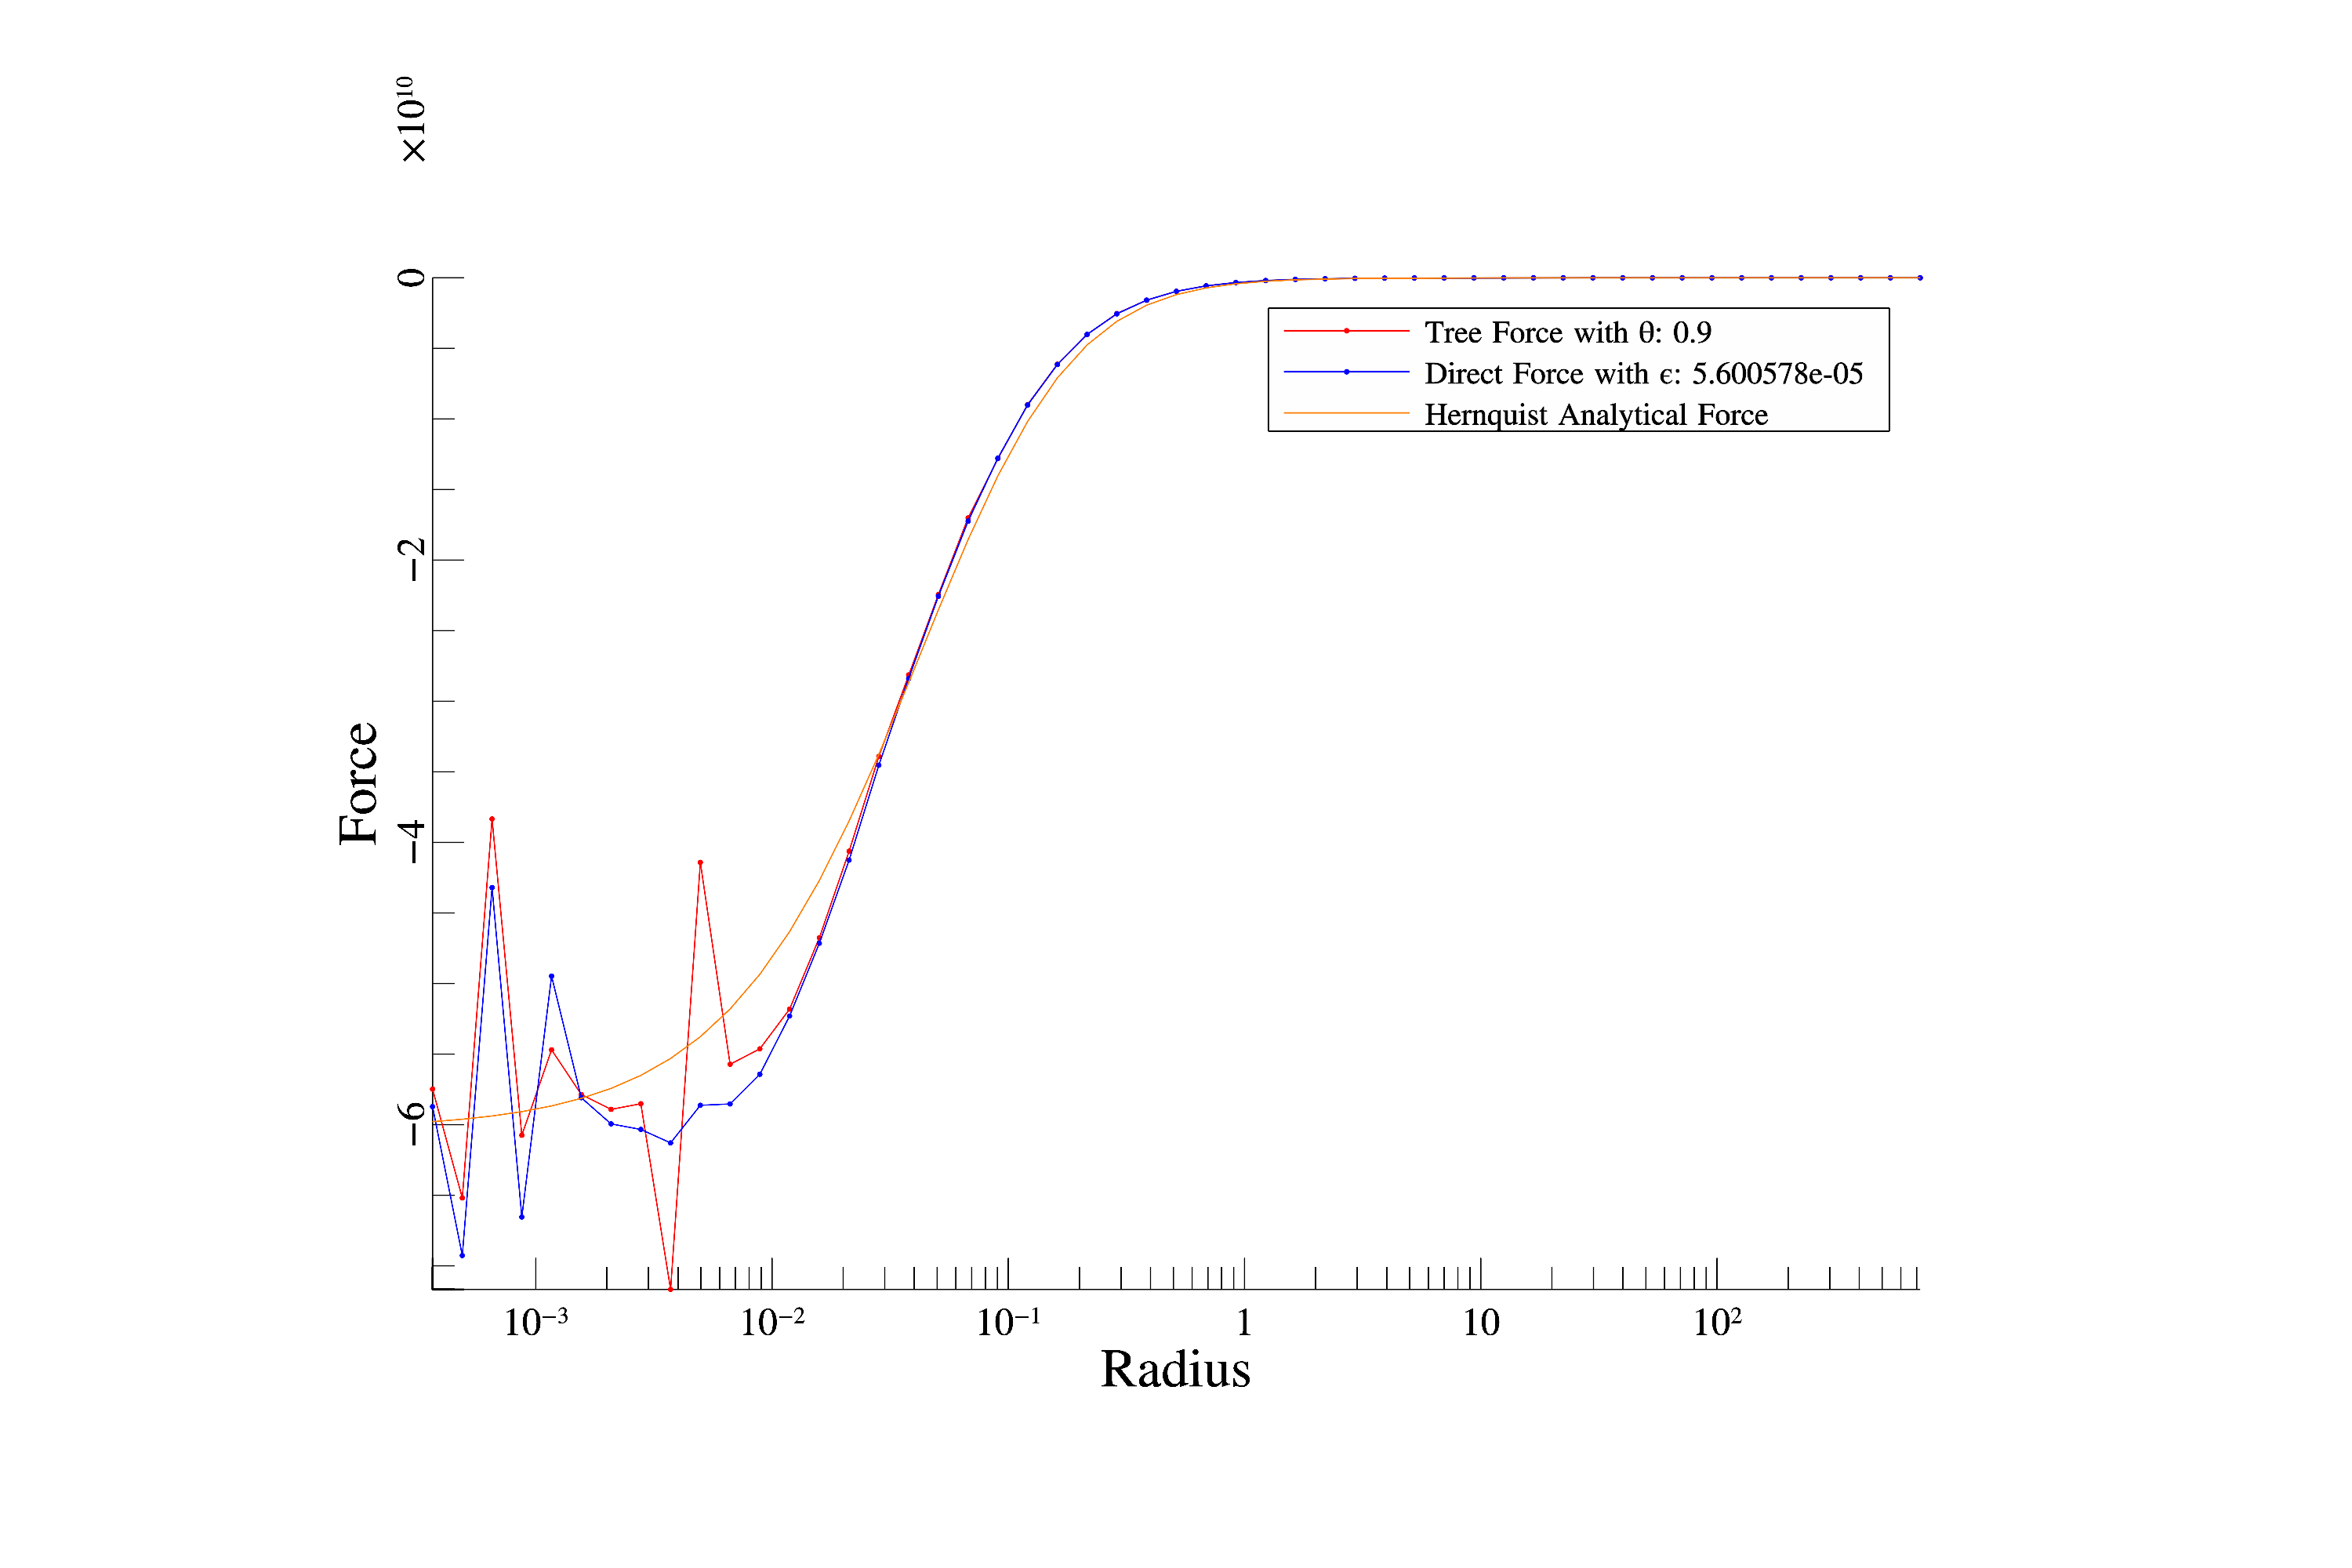
\includegraphics[width=\textwidth]{figures/plots/tree_force_0.9.png}
	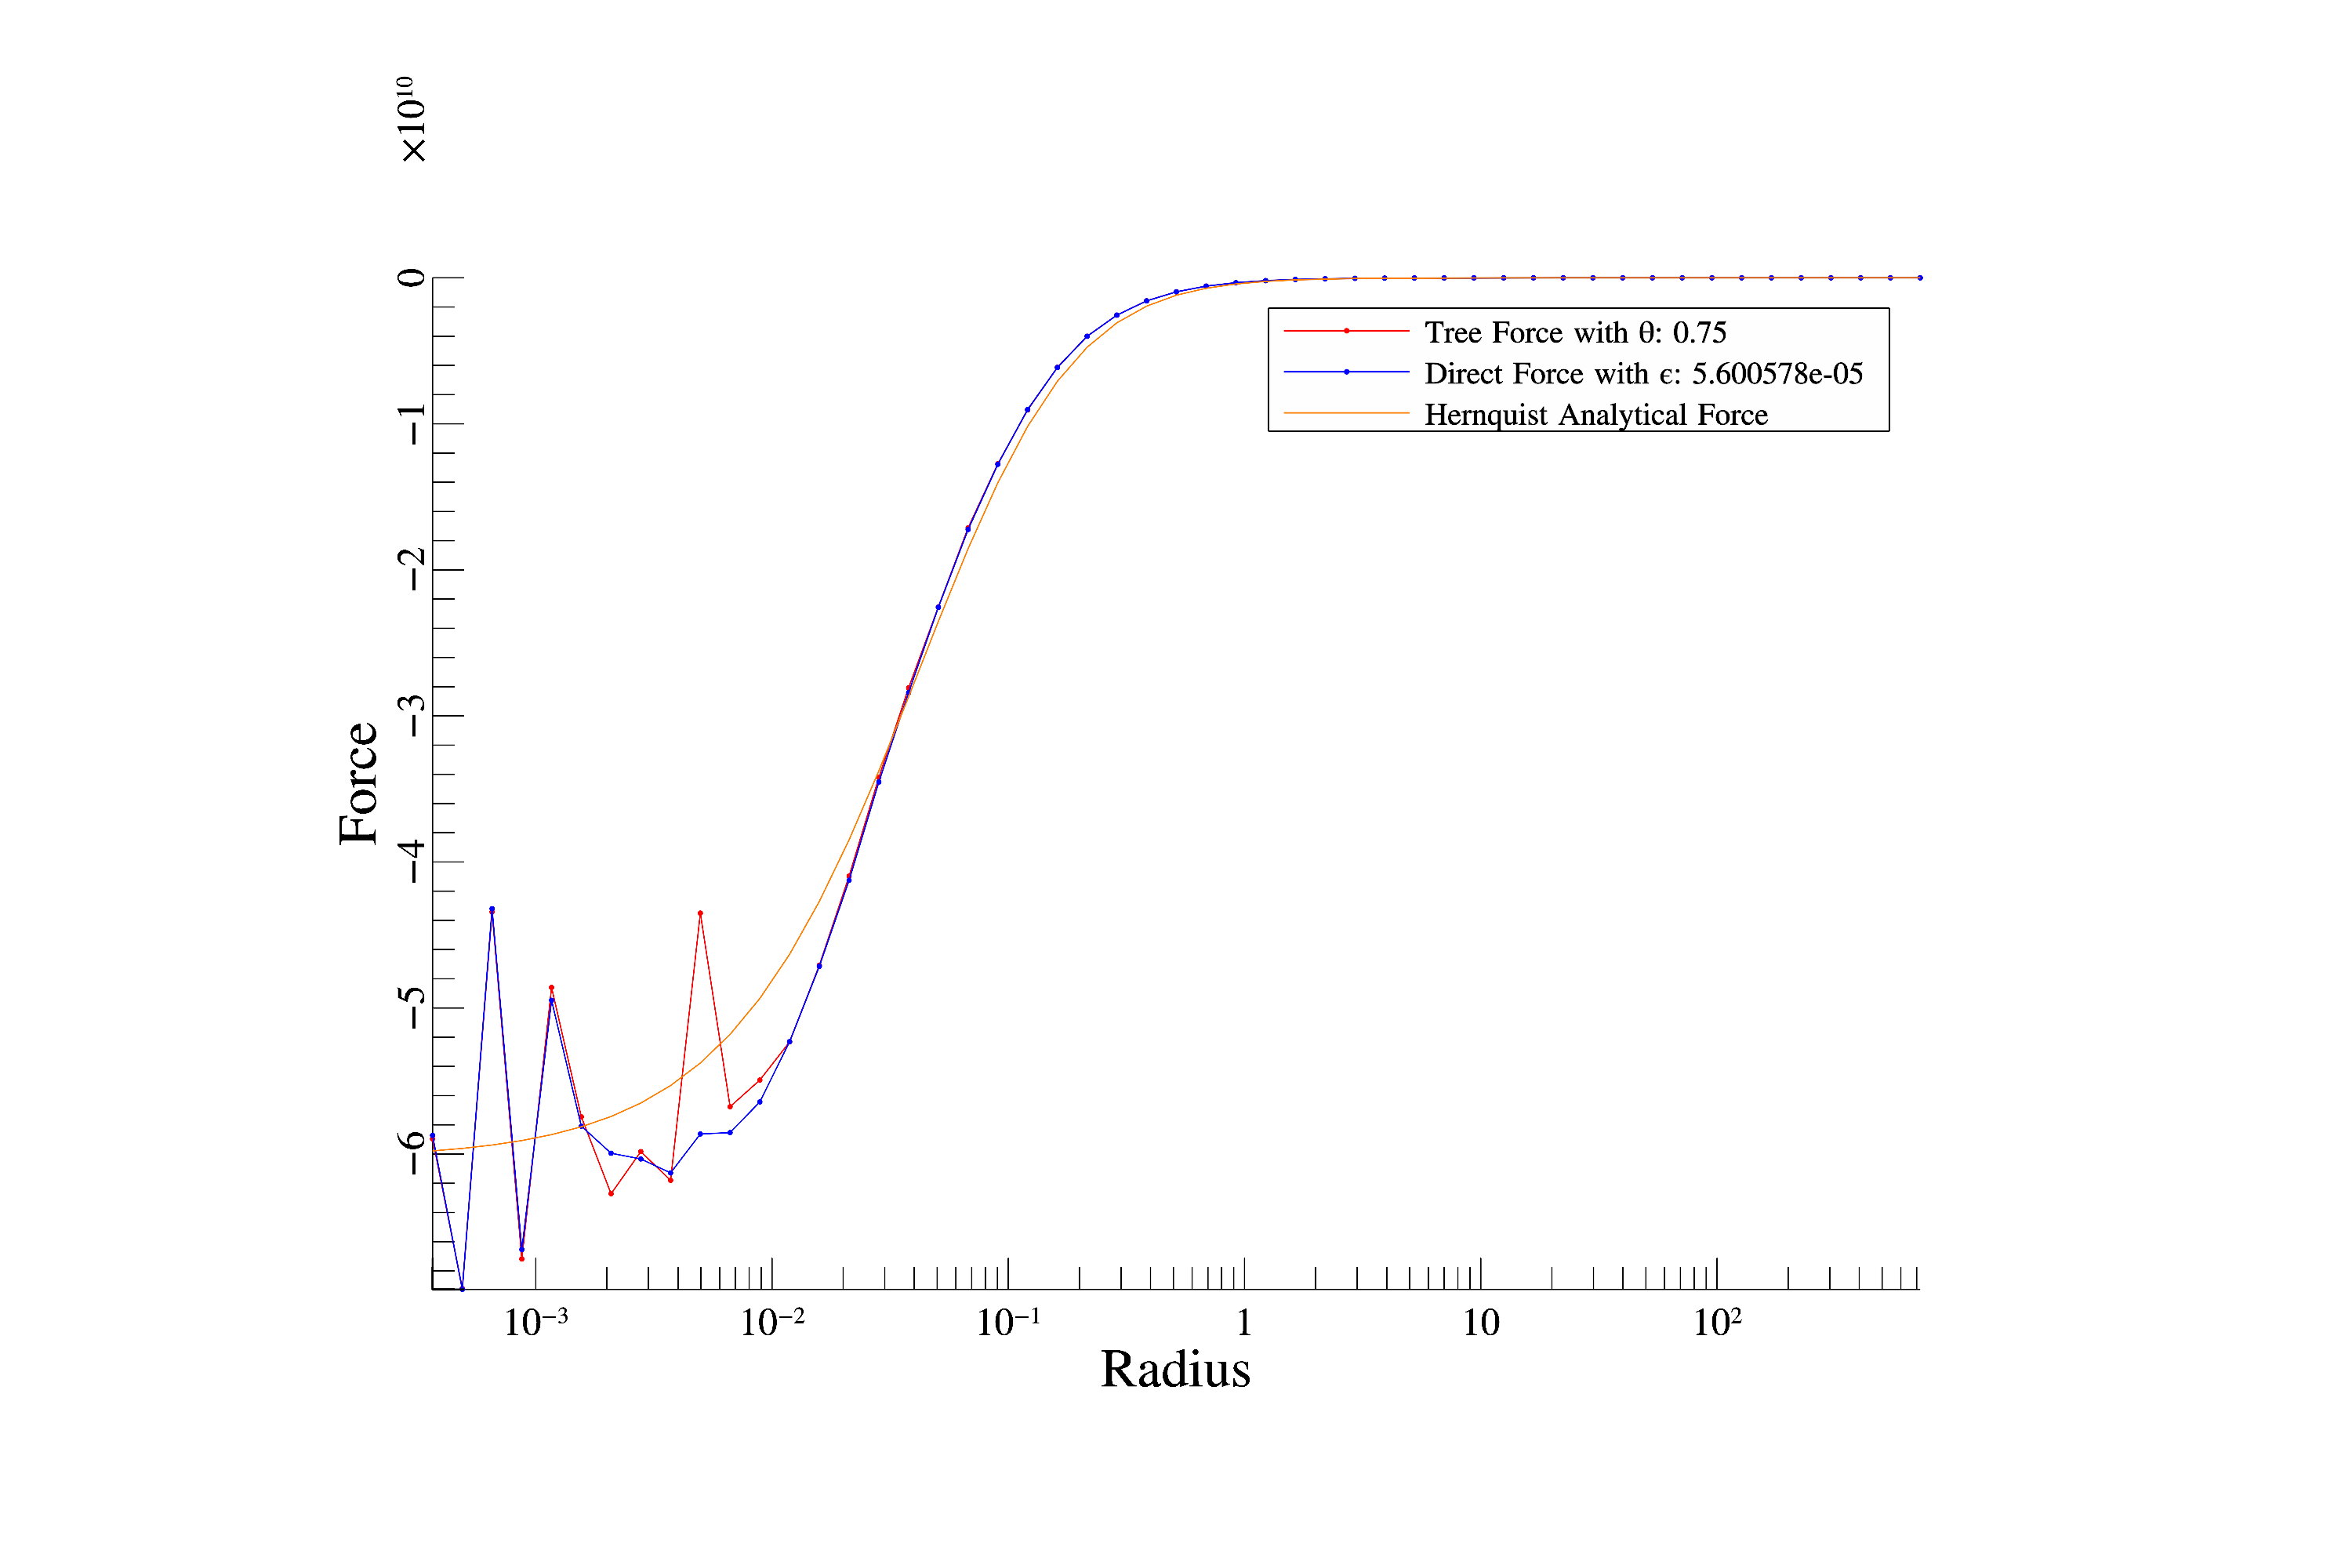
\includegraphics[width=\textwidth]{figures/plots/tree_force_0.75.png}
	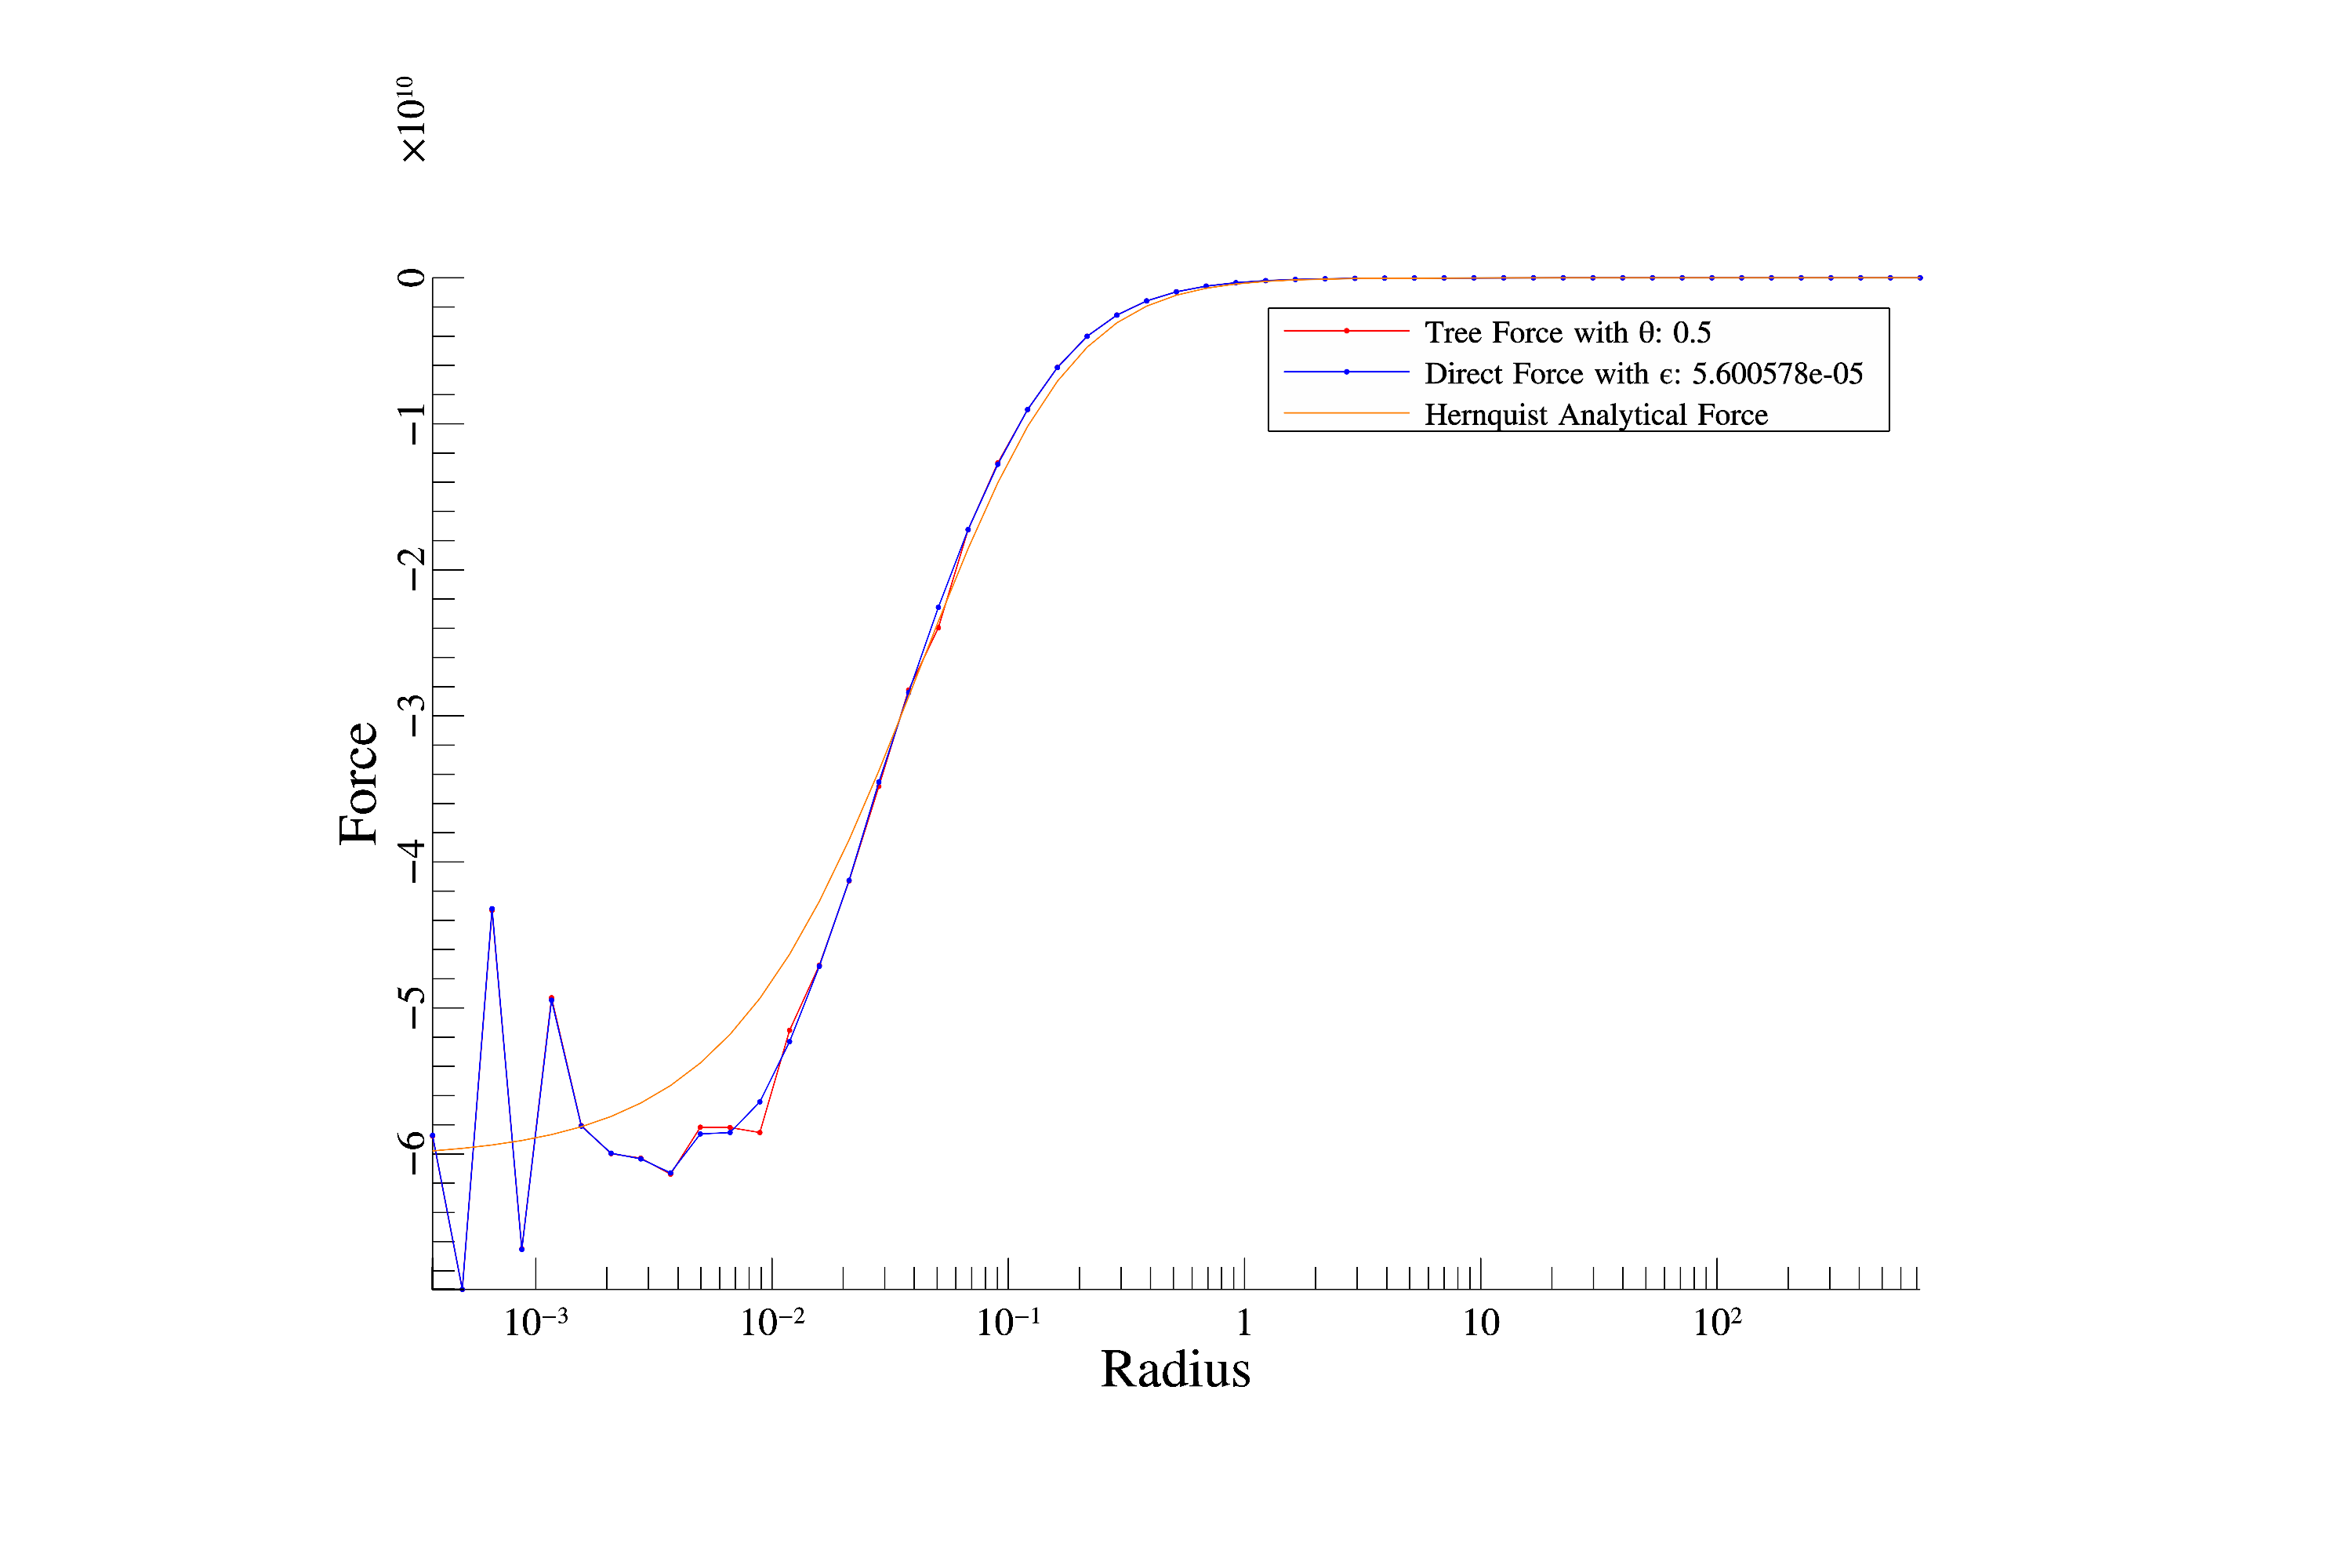
\includegraphics[width=\textwidth]{figures/plots/tree_force_0.5.png}
	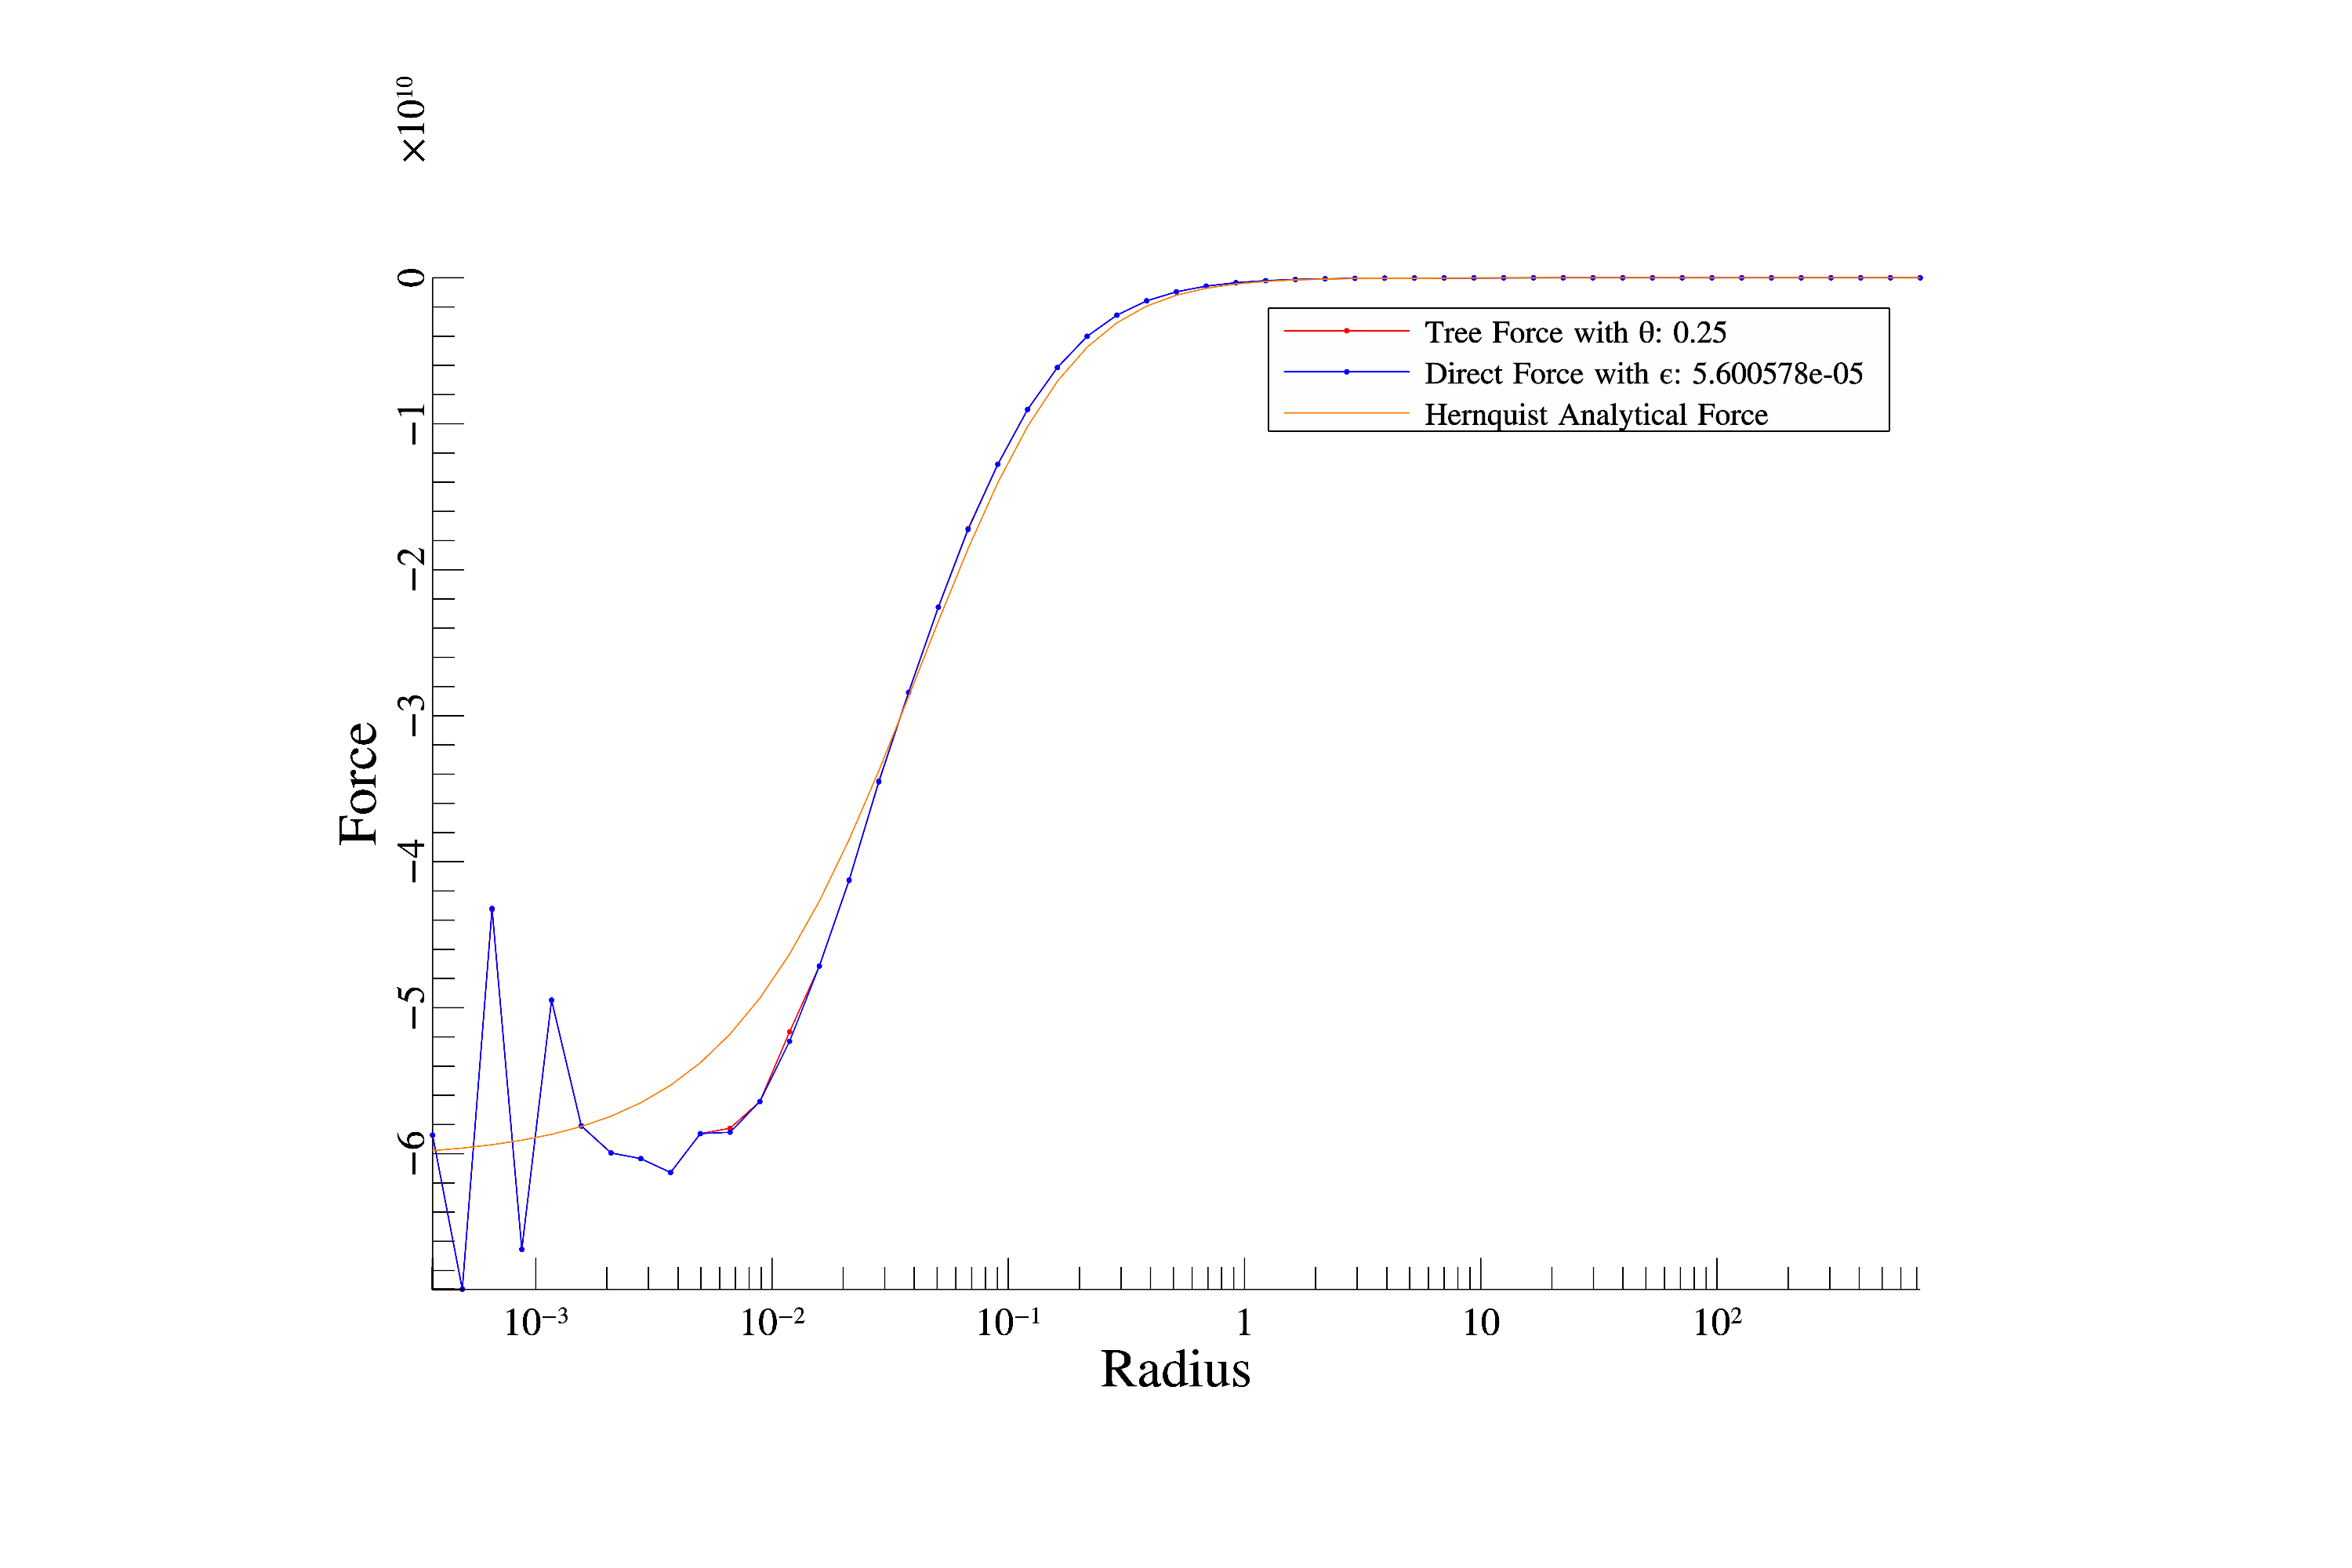
\includegraphics[width=\textwidth]{figures/plots/tree_force_0.25.png}
	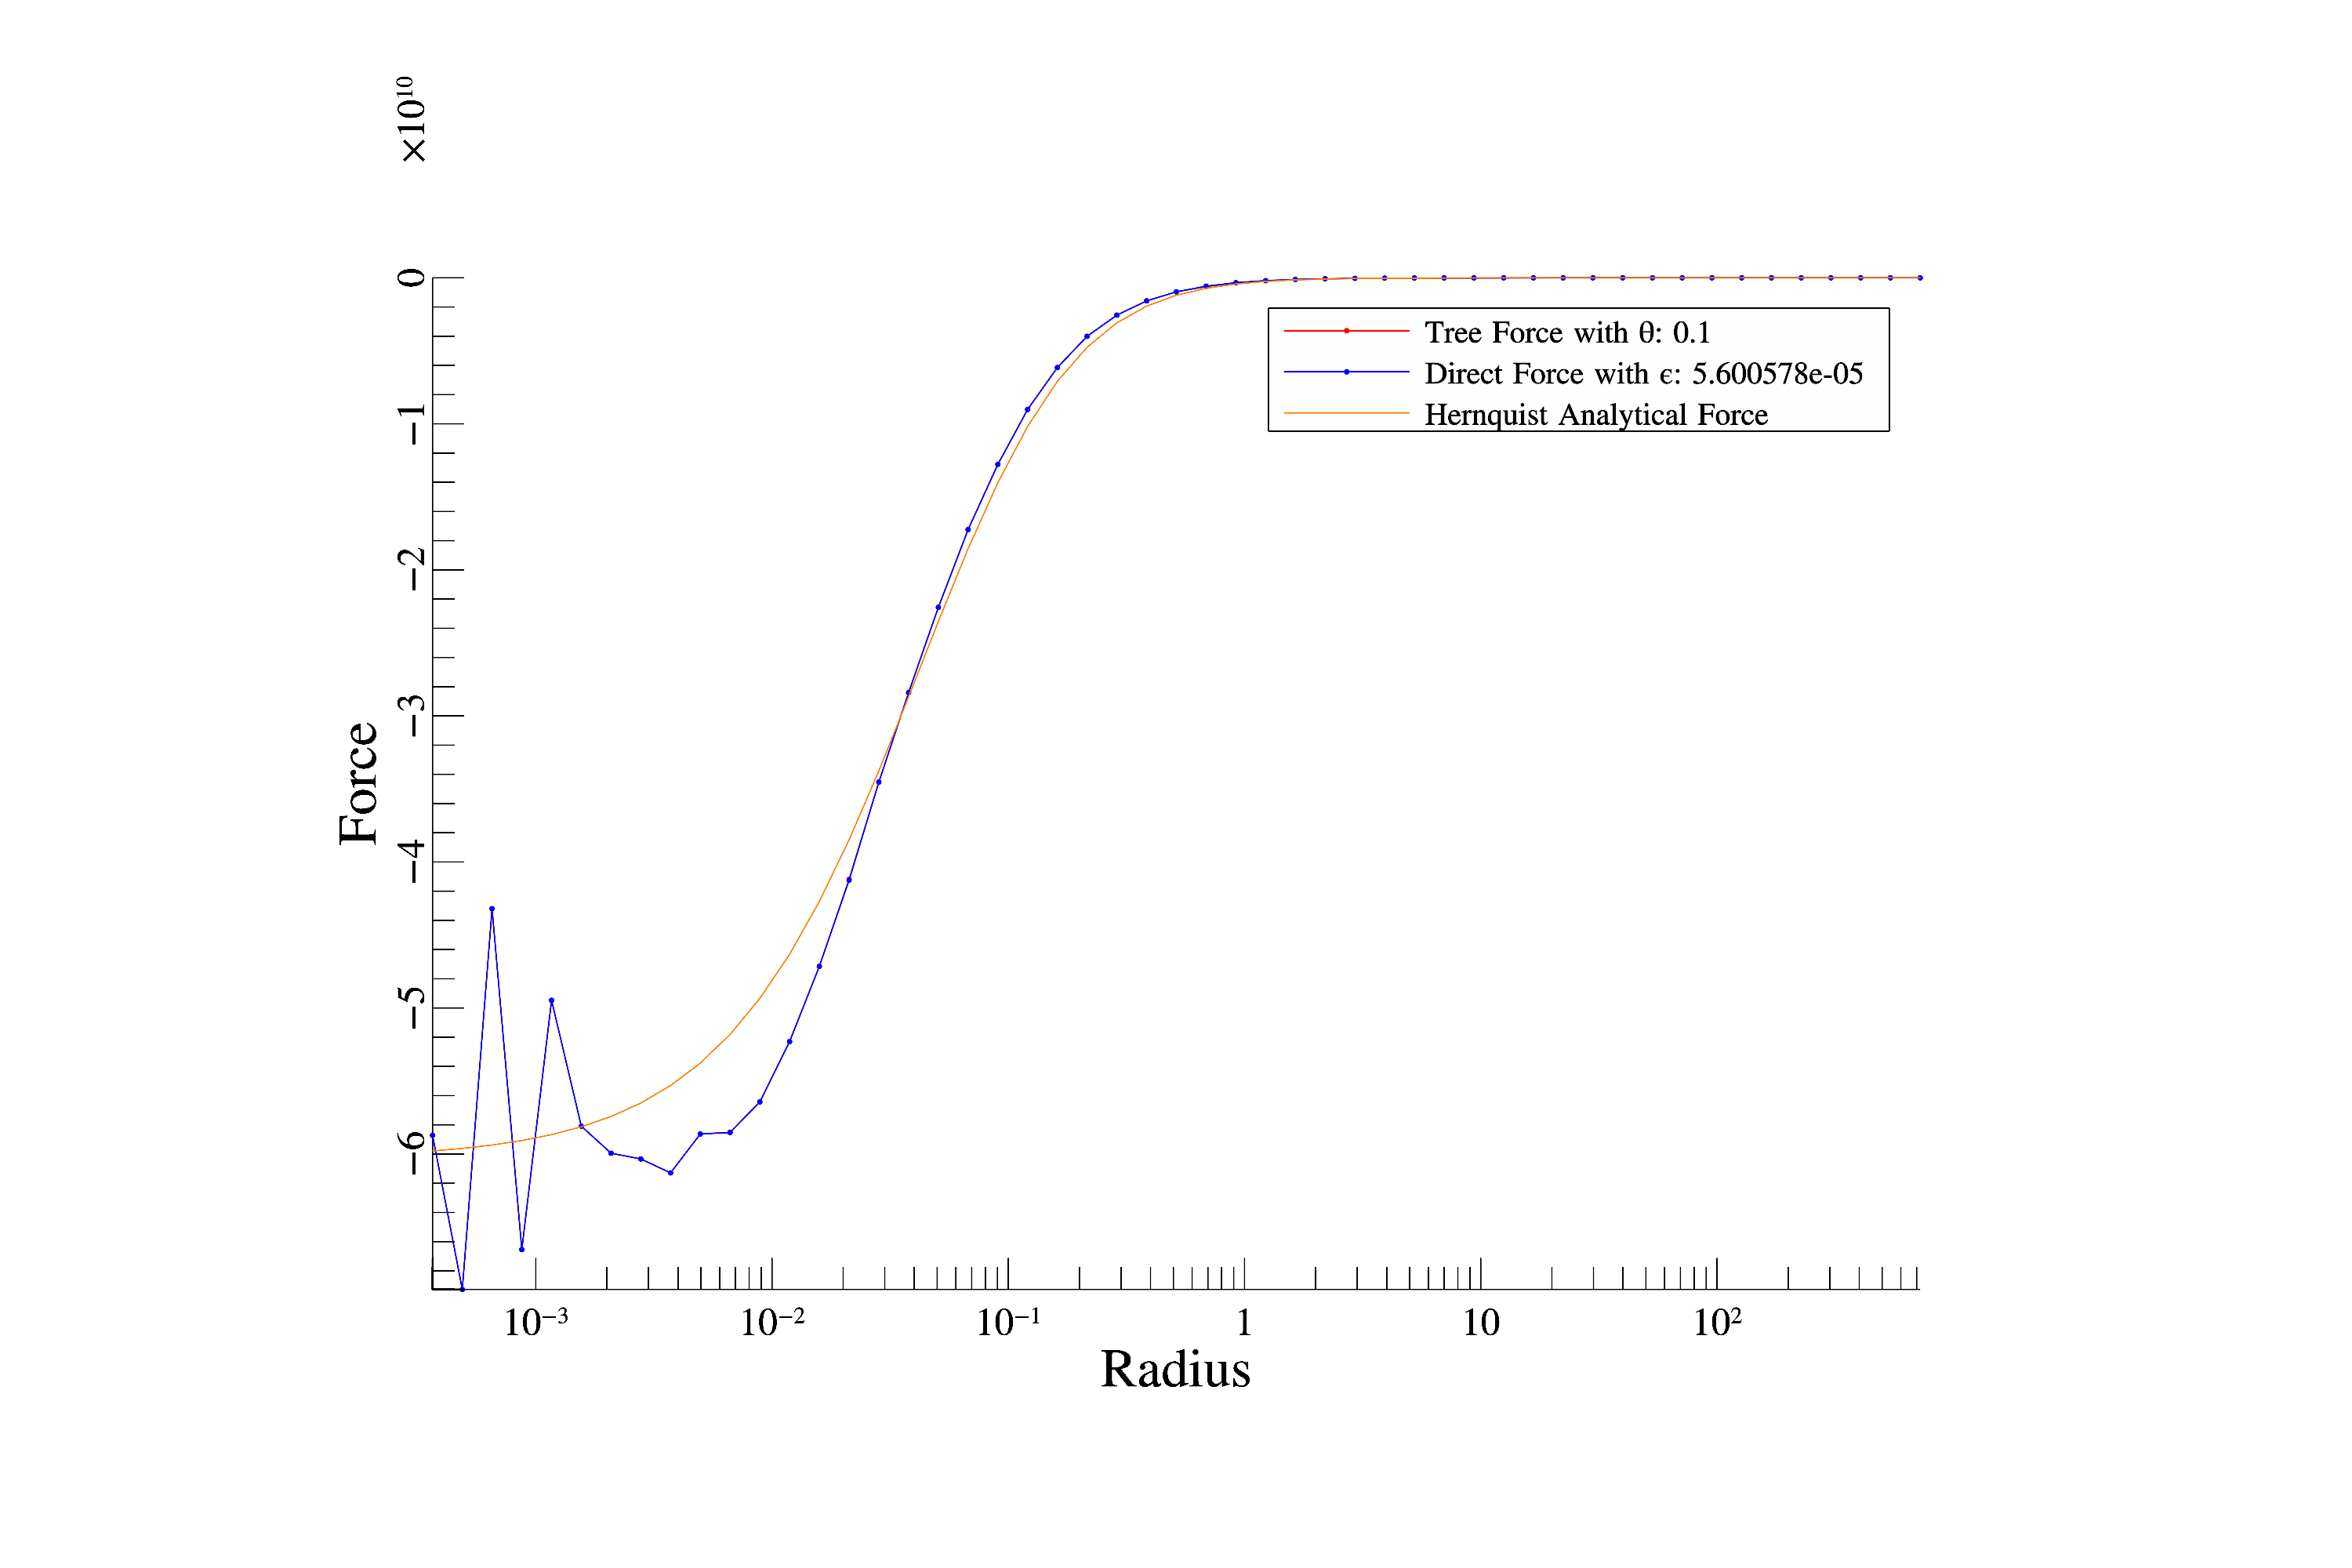
\includegraphics[width=\textwidth]{figures/plots/tree_force_0.1.png}
\end{frame}

\begin{frame}{Computational Cost Comparison}
	Direct Force Computation:
	\begin{itemize}
		\item $\mathcal{O}(N^2)$ - Comparison of each particle with every other, parallelizable
		\item $\frac{N^2}{2}$ - Comparison of each particle only with unvisited particles, not parallelizable
	\end{itemize} \bigskip


	Tree Force Computation:
	\begin{equation}
		% number of nodes needed for calculating the force on a central particle in the middle of the sphere
		N_{nodes}=\frac{4 \pi}{\theta_c^3} \ln \frac{R}{d} \propto \frac{\ln N}{\theta_c^3} .
	\end{equation}
	Expected $\mathcal{O}(N\log{N})$ but in practice values near $\approx\frac{N^2}{10'000}$
\end{frame}


%----------------------------------------------------------------------------------------
%	CLOSING SLIDE
%----------------------------------------------------------------------------------------

\section{Discussion}
\begin{frame}[plain] % The optional argument 'plain' hides the headline and footline
	\begin{center}
		{\Huge Discussion}\bigskip\bigskip

		{\LARGE Questions?}\bigskip\bigskip

		Source Code: \\
		\url{https://github.com/arminveres/comp-astro-hs23}
	\end{center}
\end{frame}
%----------------------------------------------------------------------------------------

\section{References}
\begin{frame}[allowframebreaks]{References}
	\bibliography{refs}
	\bibliographystyle{abbrv}
	\nocite{*}
\end{frame}


\end{document}
